\PassOptionsToPackage{unicode=true}{hyperref} % options for packages loaded elsewhere
\PassOptionsToPackage{hyphens}{url}
\documentclass[12pt,ignorenonframetext,]{beamer}
\IfFileExists{pgfpages.sty}{\usepackage{pgfpages}}{}
\setbeamertemplate{caption}[numbered]
\setbeamertemplate{caption label separator}{: }
\setbeamercolor{caption name}{fg=normal text.fg}
\beamertemplatenavigationsymbolsempty
\setbeameroption{show notes}
\usepackage{lmodern}
\usepackage{amssymb,amsmath}
\usepackage{ifxetex,ifluatex}
\usepackage{fixltx2e} % provides \textsubscript
\ifnum 0\ifxetex 1\fi\ifluatex 1\fi=0 % if pdftex
  \usepackage[T1]{fontenc}
  \usepackage[utf8]{inputenc}
\else % if luatex or xelatex
  \ifxetex
    \usepackage{mathspec}
  \else
    \usepackage{fontspec}
\fi
\defaultfontfeatures{Ligatures=TeX,Scale=MatchLowercase}







\fi

  \usetheme[]{metropolis}






% use upquote if available, for straight quotes in verbatim environments
\IfFileExists{upquote.sty}{\usepackage{upquote}}{}
% use microtype if available
\IfFileExists{microtype.sty}{%
  \usepackage{microtype}
  \UseMicrotypeSet[protrusion]{basicmath} % disable protrusion for tt fonts
}{}


\newif\ifbibliography
  \usepackage[round]{natbib}
  \bibliographystyle{plainnat}


\hypersetup{
      pdftitle={Machine Learning in R},
        pdfauthor={Kasun Bandara},
          pdfborder={0 0 0},
    breaklinks=true}
%\urlstyle{same}  % Use monospace font for urls




  \usepackage{color}
  \usepackage{fancyvrb}
  \newcommand{\VerbBar}{|}
  \newcommand{\VERB}{\Verb[commandchars=\\\{\}]}
  \DefineVerbatimEnvironment{Highlighting}{Verbatim}{commandchars=\\\{\}}
  % Add ',fontsize=\small' for more characters per line
  \usepackage{framed}
  \definecolor{shadecolor}{RGB}{248,248,248}
  \newenvironment{Shaded}{\begin{snugshade}}{\end{snugshade}}
  \newcommand{\AlertTok}[1]{\textcolor[rgb]{0.94,0.16,0.16}{#1}}
  \newcommand{\AnnotationTok}[1]{\textcolor[rgb]{0.56,0.35,0.01}{\textbf{\textit{#1}}}}
  \newcommand{\AttributeTok}[1]{\textcolor[rgb]{0.77,0.63,0.00}{#1}}
  \newcommand{\BaseNTok}[1]{\textcolor[rgb]{0.00,0.00,0.81}{#1}}
  \newcommand{\BuiltInTok}[1]{#1}
  \newcommand{\CharTok}[1]{\textcolor[rgb]{0.31,0.60,0.02}{#1}}
  \newcommand{\CommentTok}[1]{\textcolor[rgb]{0.56,0.35,0.01}{\textit{#1}}}
  \newcommand{\CommentVarTok}[1]{\textcolor[rgb]{0.56,0.35,0.01}{\textbf{\textit{#1}}}}
  \newcommand{\ConstantTok}[1]{\textcolor[rgb]{0.00,0.00,0.00}{#1}}
  \newcommand{\ControlFlowTok}[1]{\textcolor[rgb]{0.13,0.29,0.53}{\textbf{#1}}}
  \newcommand{\DataTypeTok}[1]{\textcolor[rgb]{0.13,0.29,0.53}{#1}}
  \newcommand{\DecValTok}[1]{\textcolor[rgb]{0.00,0.00,0.81}{#1}}
  \newcommand{\DocumentationTok}[1]{\textcolor[rgb]{0.56,0.35,0.01}{\textbf{\textit{#1}}}}
  \newcommand{\ErrorTok}[1]{\textcolor[rgb]{0.64,0.00,0.00}{\textbf{#1}}}
  \newcommand{\ExtensionTok}[1]{#1}
  \newcommand{\FloatTok}[1]{\textcolor[rgb]{0.00,0.00,0.81}{#1}}
  \newcommand{\FunctionTok}[1]{\textcolor[rgb]{0.00,0.00,0.00}{#1}}
  \newcommand{\ImportTok}[1]{#1}
  \newcommand{\InformationTok}[1]{\textcolor[rgb]{0.56,0.35,0.01}{\textbf{\textit{#1}}}}
  \newcommand{\KeywordTok}[1]{\textcolor[rgb]{0.13,0.29,0.53}{\textbf{#1}}}
  \newcommand{\NormalTok}[1]{#1}
  \newcommand{\OperatorTok}[1]{\textcolor[rgb]{0.81,0.36,0.00}{\textbf{#1}}}
  \newcommand{\OtherTok}[1]{\textcolor[rgb]{0.56,0.35,0.01}{#1}}
  \newcommand{\PreprocessorTok}[1]{\textcolor[rgb]{0.56,0.35,0.01}{\textit{#1}}}
  \newcommand{\RegionMarkerTok}[1]{#1}
  \newcommand{\SpecialCharTok}[1]{\textcolor[rgb]{0.00,0.00,0.00}{#1}}
  \newcommand{\SpecialStringTok}[1]{\textcolor[rgb]{0.31,0.60,0.02}{#1}}
  \newcommand{\StringTok}[1]{\textcolor[rgb]{0.31,0.60,0.02}{#1}}
  \newcommand{\VariableTok}[1]{\textcolor[rgb]{0.00,0.00,0.00}{#1}}
  \newcommand{\VerbatimStringTok}[1]{\textcolor[rgb]{0.31,0.60,0.02}{#1}}
  \newcommand{\WarningTok}[1]{\textcolor[rgb]{0.56,0.35,0.01}{\textbf{\textit{#1}}}}



% Prevent slide breaks in the middle of a paragraph:
\widowpenalties 1 10000
\raggedbottom

  \AtBeginPart{
    \let\insertpartnumber\relax
    \let\partname\relax
    \frame{\partpage}
  }
  \AtBeginSection{
    \ifbibliography
    \else
      \let\insertsectionnumber\relax
      \let\sectionname\relax
      \frame{\sectionpage}
    \fi
  }
  \AtBeginSubsection{
    \let\insertsubsectionnumber\relax
    \let\subsectionname\relax
    \frame{\subsectionpage}
  }



\setlength{\parindent}{0pt}
\setlength{\parskip}{6pt plus 2pt minus 1pt}
\setlength{\emergencystretch}{3em}  % prevent overfull lines
\providecommand{\tightlist}{%
  \setlength{\itemsep}{0pt}\setlength{\parskip}{0pt}}

  \setcounter{secnumdepth}{0}


  \usepackage{subfig}

  \title[]{Machine Learning in R}

  \subtitle{R-Ladies Colombo}

  \author[
        Kasun Bandara
    ]{Kasun Bandara}

  \institute[
    ]{
    Melbourne Centre for Data Science, University of Melbourne, Australia.
    }

\date[
      29 March, 2021
  ]{
      29 March, 2021
        }


\begin{document}

% Hide progress bar and footline on titlepage
  \begin{frame}[plain]
  \titlepage
  \end{frame}



\begin{frame}

\begin{figure}

\includegraphics[scale=0.22]{images/kasun}
\end{figure}

\end{frame}

\hypertarget{introduction}{%
\section{Introduction}\label{introduction}}

\begin{frame}{About me}
\protect\hypertarget{about-me}{}

\begin{itemize}
\tightlist
\item
  2015 Graduated in Computer Science from University of Colombo School
  of Computing
\item
  2015 Joined WSO2 Inc.~as a Software Engineer
\item
  2016-2020 Ph.D.~in Computer Science, Monash University, Australia

  \begin{itemize}
  \tightlist
  \item
    Topic: Forecasting In Big Data With Recurrent Neural Networks
  \item
    Machine Learning for Time Series Forecasting
  \item
    Research Internship at Walmart Labs, San Francisco, USA
  \item
    Research Scientist at Turning Point, Melbourne, Australia
  \item
    Data Science Tutor, Faculty of IT, Monash University
  \end{itemize}
\item
  2021 Research Fellow, University of Melbourne
\end{itemize}

\end{frame}

\begin{frame}{About me (2)}
\protect\hypertarget{about-me-2}{}

\begin{itemize}
\tightlist
\item
  Research Interests

  \begin{itemize}
  \tightlist
  \item
    Global Forecasting Models
  \item
    Hierarchical Forecasting
  \item
    Retail sales/demand forecasting
  \item
    Renewable energy production forecasting (solar)
  \end{itemize}
\item
  Competition Fanatic

  \begin{itemize}
  \tightlist
  \item
    M5 Forecasting Competition (\textbf{Gold Medalist})
  \item
    IEEE CIS Energy Forecasting Competition (\textbf{4th Place})
  \item
    Air-Liquide Energy Forecasting Competition (\textbf{4th Place})
  \item
    ANZ Customer Segmentation Challenge (\textbf{Top Performer})
  \end{itemize}
\end{itemize}

\end{frame}

\begin{frame}{What is Data Science ?}
\protect\hypertarget{what-is-data-science}{}

Data Science is an interdisciplinary field that permits you to extract
information from organized or unstructured data.

\begin{figure}
  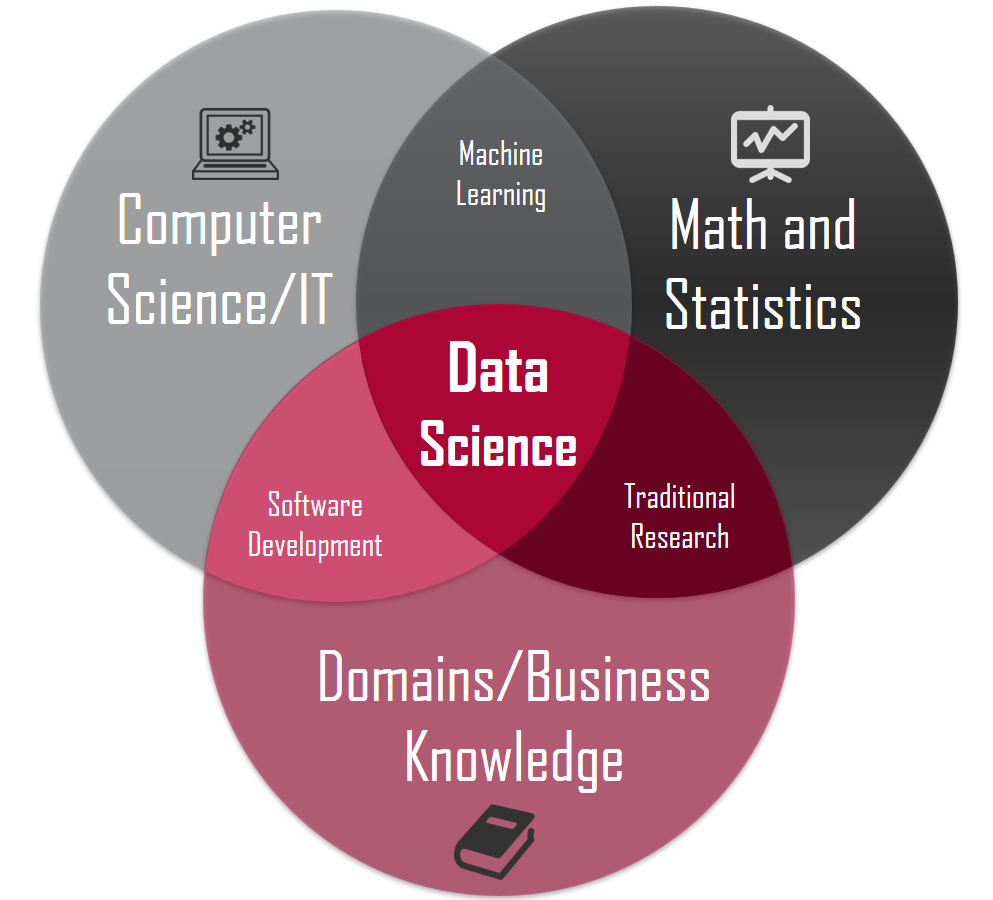
\includegraphics[width=.5\textwidth,height=.5\textheight,keepaspectratio]{images/datascience.jpeg}
  \caption{An intersection of many fields of science%
    \footnote{%
     \tiny{Image source: https://medium.com/believing-these-8-myths-about-what-is-data-science-keeps-you-from-growing-528f1bd240dc} 
    }%
  }
\end{figure}

\end{frame}

\begin{frame}{Data Science Life Cycle}
\protect\hypertarget{data-science-life-cycle}{}

Known as the O.S.E.M.N. framework.

\begin{figure}
  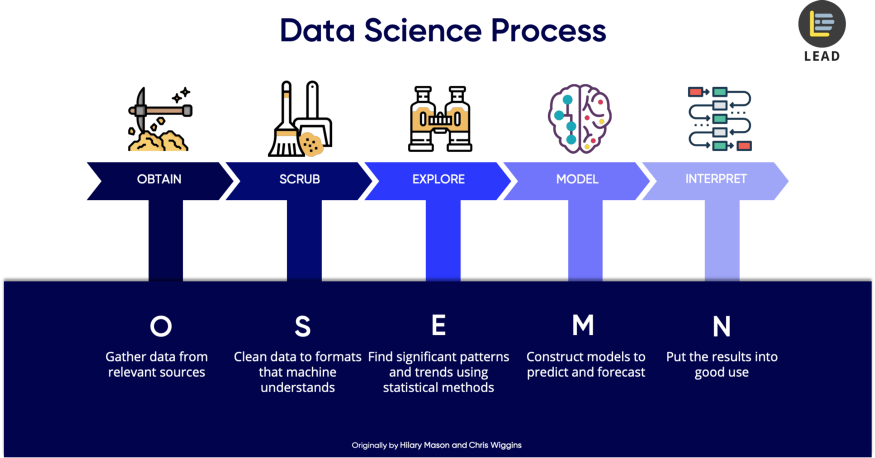
\includegraphics[width=.8\textwidth,height=.8\textheight,keepaspectratio]{images/osemn.png}
  \caption{Data Science Process%
    \footnote{%
     \tiny{Image source: https://towardsdatascience.com/5-steps-of-a-data-science-project-lifecycle-26c50372b492} 
    }%
  }
\end{figure}

\end{frame}

\begin{frame}{Obtain (O)}
\protect\hypertarget{obtain-o}{}

\begin{itemize}
\tightlist
\item
  Retrieving data from multiple sources of inputs.\\

  \begin{itemize}
      \item Structured Data: RDBMS, Tabular Data, CSV, TSV.
      \item Unstructured Data: NoSQL Databases, API Data (Twitter, Facebook).
  \end{itemize}
   \vspace{2mm}
\item
  Databases: \texttt{\{odbc\}} \vspace{2mm}
\item
  Scraping data from websites: \texttt{\{rvest\}} \vspace{2mm}
\item
  Data platforms: \textbf{Kaggle}, \textbf{UCI}, \textbf{Competition
  Datasets}, \textbf{Government APIs}
\end{itemize}

\end{frame}

\begin{frame}[fragile]{Example of \texttt{\{rvest\}}}
\protect\hypertarget{example-of}{}

\tiny

\begin{Shaded}
\begin{Highlighting}[]
\KeywordTok{library}\NormalTok{(rvest)}
\KeywordTok{library}\NormalTok{(dplyr)}
\KeywordTok{set.seed}\NormalTok{(}\DecValTok{1234}\NormalTok{)}

\CommentTok{# reading the HTML page (Lord of the Rings)}
\NormalTok{lor_movie <-}\StringTok{ }\KeywordTok{read_html}\NormalTok{(}\StringTok{"https://www.imdb.com/title/tt0120737/"}\NormalTok{)}

\CommentTok{# Scraping the movie rating.}
\NormalTok{lor_movie }\OperatorTok
\StringTok{  }\KeywordTok{html_node}\NormalTok{(}\StringTok{"strong span"}\NormalTok{) }\OperatorTok
\StringTok{  }\KeywordTok{html_text}\NormalTok{() }\OperatorTok
\StringTok{  }\KeywordTok{as.numeric}\NormalTok{()}
\CommentTok{#[1] 8.8}

\CommentTok{# Scraping the cast.}
\NormalTok{lor_movie }\OperatorTok
\StringTok{  }\KeywordTok{html_nodes}\NormalTok{(}\StringTok{"#titleCast .itemprop span"}\NormalTok{) }\OperatorTok
\StringTok{  }\KeywordTok{html_text}\NormalTok{()}

\CommentTok{# Scraping the movie poster.}
\NormalTok{lor_movie }\OperatorTok
\StringTok{  }\KeywordTok{html_nodes}\NormalTok{(}\StringTok{"#img_primary img"}\NormalTok{) }\OperatorTok
\StringTok{  }\KeywordTok{html_attr}\NormalTok{(}\StringTok{"src"}\NormalTok{)}
\end{Highlighting}
\end{Shaded}

\normalsize

\end{frame}

\begin{frame}{Scrub (S)}
\protect\hypertarget{scrub-s}{}

\begin{itemize}
\tightlist
\item
  Also known as \textbf{data pre-processing}, \textbf{data wrangling}.\\
  \vspace{2mm}
\item
  Converting the data into a unified, suitable format

  \begin{itemize}
      \item Easier for the data exploration process.
      \item What your predictive algorithm expects ?
      \item \textbf{tidyverse} \texttt{\{dplyr,tidyr,stringr,tibble,purr,ggplot2\}}
  \end{itemize}
   \vspace{2mm}
\item
  Handles data issues

  \begin{itemize}
      \item Cleaning: Missing values, Outliers, Noisy data.
      \item Transformation: Normalisation, Feature Discretization.
      \item Reduction: Feature selection, Dimensionality reduction.
  \end{itemize}
\end{itemize}

\end{frame}

\begin{frame}[fragile]{Missing Value Imputation}
\protect\hypertarget{missing-value-imputation}{}

\tiny

\begin{Shaded}
\begin{Highlighting}[]
\KeywordTok{library}\NormalTok{(simputation)}
\KeywordTok{set.seed}\NormalTok{(}\DecValTok{1234}\NormalTok{)}

\CommentTok{# Loading iris dataset and randomly inserting NAs.}
\NormalTok{df <-}\StringTok{ }\NormalTok{iris}
\NormalTok{df_NA <-}\StringTok{ }\KeywordTok{as.data.frame}\NormalTok{(}\KeywordTok{lapply}\NormalTok{(df, }\ControlFlowTok{function}\NormalTok{(imp) imp[ }\KeywordTok{sample}\NormalTok{(}\KeywordTok{c}\NormalTok{(}\OtherTok{TRUE}\NormalTok{, }\OtherTok{NA}\NormalTok{), }
        \DataTypeTok{prob =} \KeywordTok{c}\NormalTok{(}\FloatTok{0.85}\NormalTok{, }\FloatTok{0.15}\NormalTok{), }\DataTypeTok{size =} \KeywordTok{length}\NormalTok{(imp), }\DataTypeTok{replace =} \OtherTok{TRUE}\NormalTok{)]))}

\CommentTok{# Using median to impute the missing values.}
\NormalTok{median_imputed <-}\StringTok{ }\KeywordTok{impute_median}\NormalTok{(df_NA, }
\NormalTok{                                Sepal.Length }\OperatorTok{~}\StringTok{ }\NormalTok{Species)}

\CommentTok{# Using linear regression to impute the missing values.}
\NormalTok{linear_imputed <-}\StringTok{ }\KeywordTok{impute_lm}\NormalTok{(df_NA, Sepal.Length }\OperatorTok{~}\StringTok{ }\NormalTok{Sepal.Width }\OperatorTok{+}\StringTok{ }\NormalTok{Species)}

\CommentTok{# Using CART algorithm to impute the missing values.}
\NormalTok{cart_imputed <-}\StringTok{ }\KeywordTok{impute_cart}\NormalTok{(df_NA, Species }\OperatorTok{~}\StringTok{ }\NormalTok{.)}

\CommentTok{# Imputing multiple variables at once.}
\NormalTok{multivariable_imputed <-}\StringTok{ }\KeywordTok{impute_rlm}\NormalTok{(df_NA, Sepal.Length }\OperatorTok{+}\StringTok{ }\NormalTok{Sepal.Width }
                                    \OperatorTok{~}\StringTok{ }\NormalTok{Petal.Length }\OperatorTok{+}\StringTok{ }\NormalTok{Species)}

\CommentTok{# Imputing using a pre-trained model.}
\NormalTok{model <-}\StringTok{ }\KeywordTok{lm}\NormalTok{(Sepal.Length }\OperatorTok{~}\StringTok{ }\NormalTok{Sepal.Width }\OperatorTok{+}\StringTok{ }\NormalTok{Species, }\DataTypeTok{data=}\NormalTok{iris)}
\NormalTok{model_imputed <-}\StringTok{ }\KeywordTok{impute}\NormalTok{(df_NA, Sepal.Length }\OperatorTok{~}\StringTok{ }\NormalTok{model)}
\end{Highlighting}
\end{Shaded}

\normalsize

\end{frame}

\begin{frame}{Dealing with Outliers}
\protect\hypertarget{dealing-with-outliers}{}

\begin{itemize}
\tightlist
\item
  A data point that differs significantly from other observations.\\
  \vspace{2mm}
\item
  Observations that distort your analysis.

  \begin{itemize}
      \item Boxplot visualisation: \texttt{\{ggplot2\}}
      \item Grubbs’s test, Dixon’s test, Rosner’s test: \texttt{\{outliers\}}
      \item Outlier detection algorithms: \texttt{\{OutlierDetection\}}
      \item \textbf{outlierTest()} from \texttt{\{car\}}
      \item \textbf{lofactor()} from \texttt{\{DMwR\}} (Local Outlier Factor)
  \end{itemize}
   \vspace{2mm}
\item
  Anomaly detection is itself a different research area !

  \begin{itemize}
      \item One Class SVM, IsolationForest
      \item Unsupervised algorithms (Clustering)
      \item Time series: \texttt{\{tsoutliers,oddstream,stray\}}
  \end{itemize}
\end{itemize}

\end{frame}

\begin{frame}{Feature Selection}
\protect\hypertarget{feature-selection}{}

\begin{itemize}
\tightlist
\item
  Removing redundant features from the dataset. \vspace{2mm}
\item
  Computational complexity, Address model overfitting. \vspace{2mm}
\item
  \textbf{Filter Methods}

  \begin{itemize}
      \item Features are selected based on a statistical score.
      \item Independent of any machine learning algorithm.
      \item \textbf{Pearson’s Correlation, Chi-Square, PCA}
  \end{itemize}
   \vspace{2mm}
\item
  \textbf{Wrapper Methods}

  \begin{itemize}
      \item A subset of features are used to train a model.
      \item Forward, Backward, Recursive elimination.
      \item Inbuilt penalization functions: \textbf{LASSO, RIDGE} regression 
      \item \texttt{\{Boruta,caret,glmnet\}}
  \end{itemize}
\end{itemize}

\end{frame}

\begin{frame}[fragile]{Using Correlation}
\protect\hypertarget{using-correlation}{}

\tiny

\begin{Shaded}
\begin{Highlighting}[]
\KeywordTok{library}\NormalTok{(GGally)}
\KeywordTok{library}\NormalTok{(dplyr)}
\KeywordTok{set.seed}\NormalTok{(}\DecValTok{1234}\NormalTok{)}

\CommentTok{# Plotting the feature correlations.}
\NormalTok{iris }\OperatorTok\StringTok{ }\KeywordTok{select}\NormalTok{(}\OperatorTok{-}\NormalTok{Species) }\OperatorTok\StringTok{ }\KeywordTok{ggpairs}\NormalTok{()}
\end{Highlighting}
\end{Shaded}

\begin{center}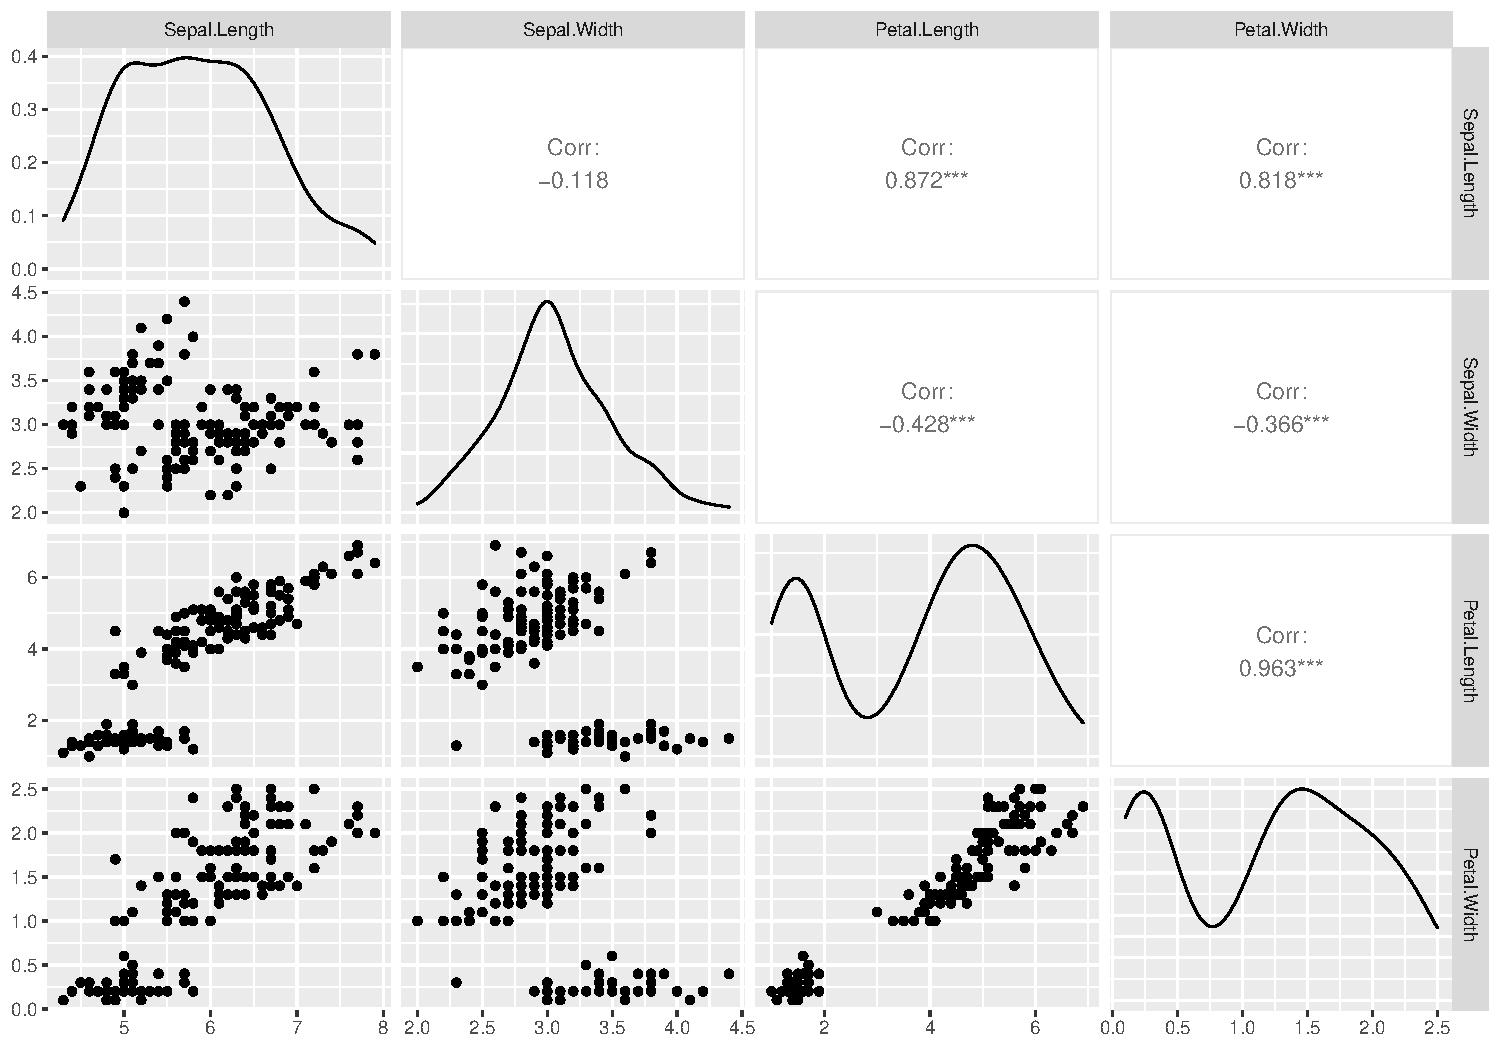
\includegraphics[width=0.7\linewidth,height=0.6\textheight]{figs/unnamed-chunk-1} \end{center}

\normalsize

\end{frame}

\begin{frame}[fragile]{Using PCR}
\protect\hypertarget{using-pcr}{}

\tiny

\begin{Shaded}
\begin{Highlighting}[]
\KeywordTok{library}\NormalTok{(dplyr)}
\KeywordTok{set.seed}\NormalTok{(}\DecValTok{1234}\NormalTok{)}

\CommentTok{# Plotting the feature importance.}
\NormalTok{pcomp_df <-}\StringTok{ }\NormalTok{iris }\OperatorTok\StringTok{ }
\StringTok{  }\KeywordTok{select}\NormalTok{(}\OperatorTok{-}\NormalTok{Species) }\OperatorTok\StringTok{ }\KeywordTok{prcomp}\NormalTok{(}\DataTypeTok{scale. =}\NormalTok{ T, }\DataTypeTok{center =}\NormalTok{ T) }\OperatorTok
\StringTok{  }\KeywordTok{plot}\NormalTok{(}\DataTypeTok{type=}\StringTok{"l"}\NormalTok{, }\DataTypeTok{main =} \StringTok{"Principle Components"}\NormalTok{)}
\end{Highlighting}
\end{Shaded}

\begin{center}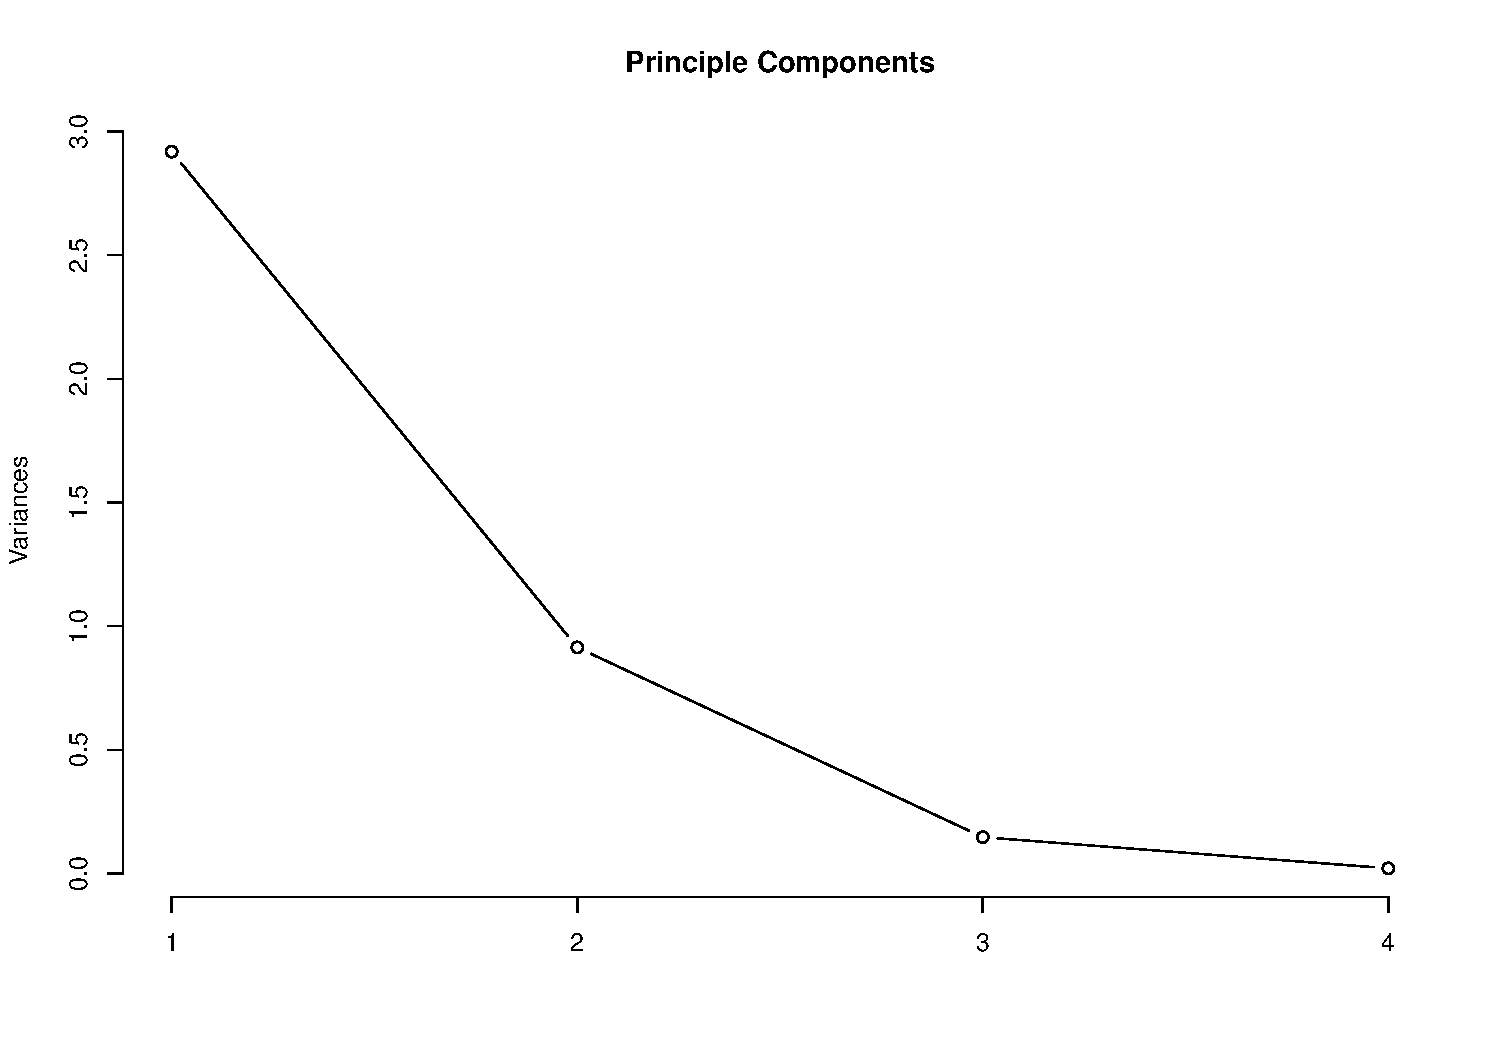
\includegraphics[width=0.7\linewidth,height=0.6\textheight]{figs/unnamed-chunk-2} \end{center}

\normalsize

\end{frame}

\begin{frame}[fragile]{Example of \texttt{\{Boruta\}}}
\protect\hypertarget{example-of-1}{}

\tiny

\begin{Shaded}
\begin{Highlighting}[]
\KeywordTok{library}\NormalTok{(Boruta)}
\KeywordTok{set.seed}\NormalTok{(}\DecValTok{1234}\NormalTok{)}

\CommentTok{# Boruta is a feature selection algorithm based on the random forests algorithm.}
\NormalTok{boruta_df <-}\StringTok{ }\KeywordTok{Boruta}\NormalTok{(Species }\OperatorTok{~}\StringTok{ }\NormalTok{., }\DataTypeTok{data=}\NormalTok{iris, }\DataTypeTok{doTrace=}\DecValTok{0}\NormalTok{)}

\CommentTok{# Plotting the feature importance.}
\KeywordTok{plot}\NormalTok{(boruta_df, }\DataTypeTok{xlab=}\StringTok{"Features"}\NormalTok{, }\DataTypeTok{main=}\StringTok{"Variable Importance"}\NormalTok{)}
\end{Highlighting}
\end{Shaded}

\begin{center}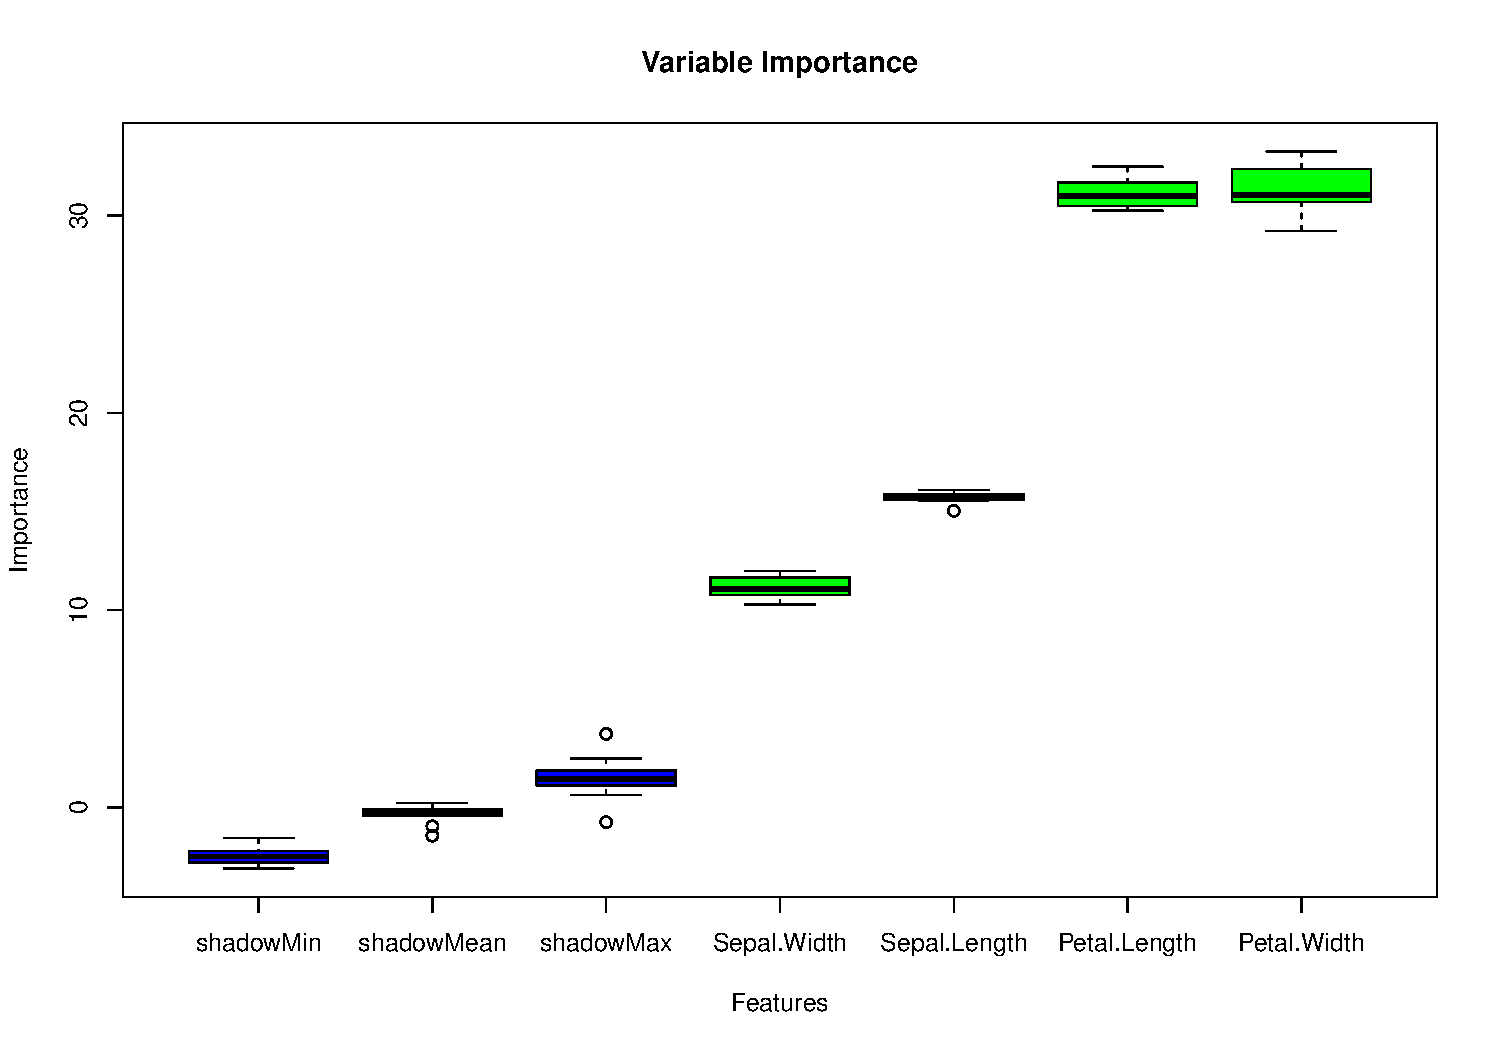
\includegraphics[width=0.7\linewidth,height=0.6\textheight]{figs/unnamed-chunk-3} \end{center}

\normalsize

\end{frame}

\begin{frame}[fragile]{Example of \texttt{\{caret\}}}
\protect\hypertarget{example-of-2}{}

\tiny

\begin{Shaded}
\begin{Highlighting}[]
\KeywordTok{library}\NormalTok{(caret)}
\KeywordTok{set.seed}\NormalTok{(}\DecValTok{1234}\NormalTok{)}

\CommentTok{# Build a decision tree model using rpart (Recursive Partitioning And Regression Trees)}
\NormalTok{rPart_df <-}\StringTok{ }\KeywordTok{train}\NormalTok{(Species }\OperatorTok{~}\StringTok{ }\NormalTok{., }\DataTypeTok{data=}\NormalTok{iris, }\DataTypeTok{method=}\StringTok{"rpart"}\NormalTok{)}
\NormalTok{rPart_imp <-}\StringTok{ }\KeywordTok{varImp}\NormalTok{(rPart_df)}

\CommentTok{# Plotting the feature importance.}
\KeywordTok{plot}\NormalTok{(rPart_imp, }\DataTypeTok{top =} \DecValTok{3}\NormalTok{, }\DataTypeTok{main=}\StringTok{'Variable Importance'}\NormalTok{, }\DataTypeTok{ylab =} \StringTok{"Features"}\NormalTok{)}
\end{Highlighting}
\end{Shaded}

\begin{center}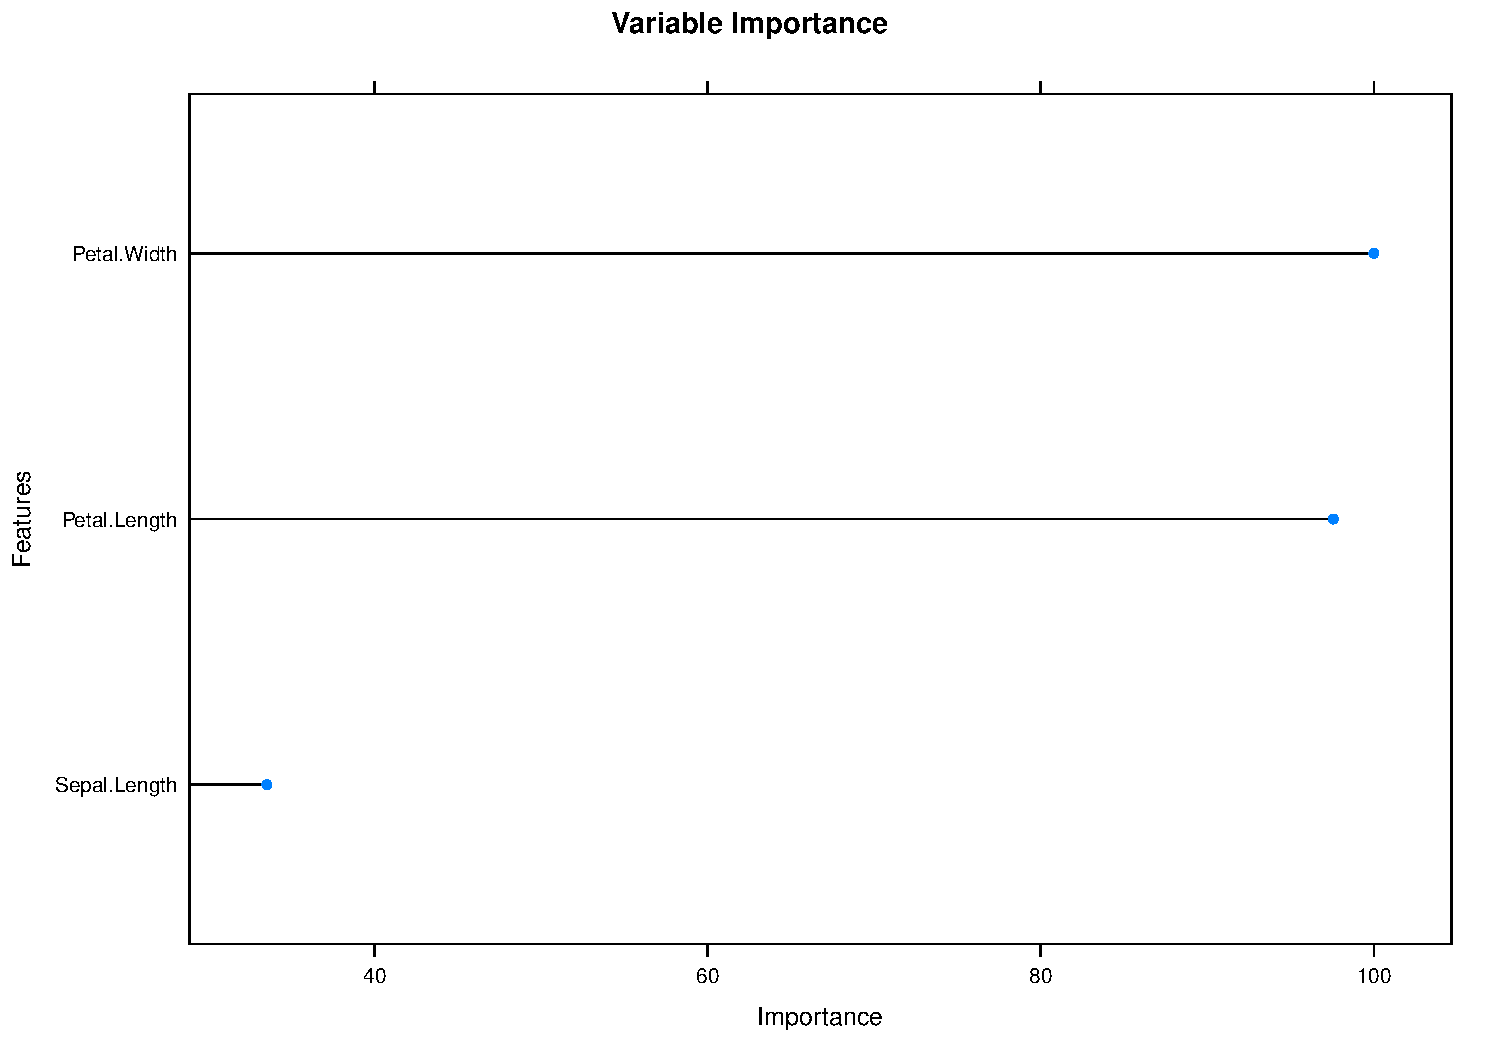
\includegraphics[width=0.7\linewidth,height=0.6\textheight]{figs/unnamed-chunk-4} \end{center}

\normalsize

\end{frame}

\begin{frame}{Explore (E)}
\protect\hypertarget{explore-e}{}

\begin{itemize}
\tightlist
\item
  Examination of data, features, and their characteristics. \vspace{2mm}

  \begin{itemize}
      \item Data types: numerical, ordinal, and nominal data.
      \item Summary statistics.
      \item Feature distributions.
      \item Feature correlations (positive, negative).
      \item Classification: class distribution (\textbf{Class Imbalance?})
  \end{itemize}
   \vspace{2mm}
\item
  Invest your time more on the data exploration process.

  \begin{itemize}
      \item Frequency distribution: \textbf{Histograms}
      \item Outlier detection: \textbf{Box plots}
      \item Feature correlation analysis: \textbf{Scatter plots}
      \item Time series analysis: \textbf{Trend and Seasonal plots}
  \end{itemize}
\end{itemize}

\end{frame}

\begin{frame}{Tools available for Exploration}
\protect\hypertarget{tools-available-for-exploration}{}

\begin{figure}
  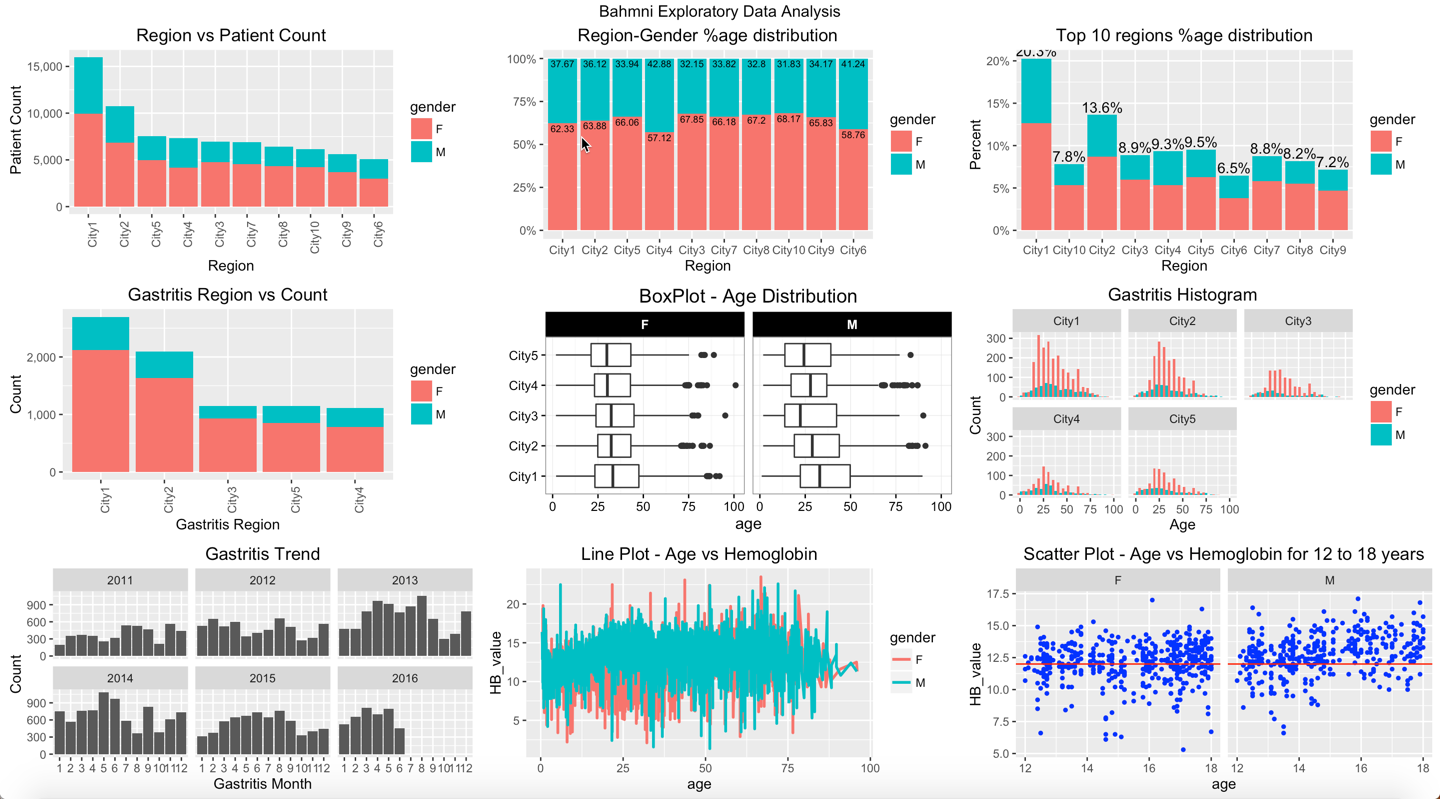
\includegraphics[width=.9\textwidth,height=.9\textheight,keepaspectratio]{images/data_exploration.png}
  \caption{Plots available from \texttt{\{ggplot2\}}%
    \footnote{%
     \tiny{Image source: https://www.pinterest.com.au/pin/281686151677624808/}
    }%
  }
\end{figure}

\end{frame}

\begin{frame}{Seasonal plot from \texttt{\{feasts\}}}
\protect\hypertarget{seasonal-plot-from}{}

\begin{figure}
  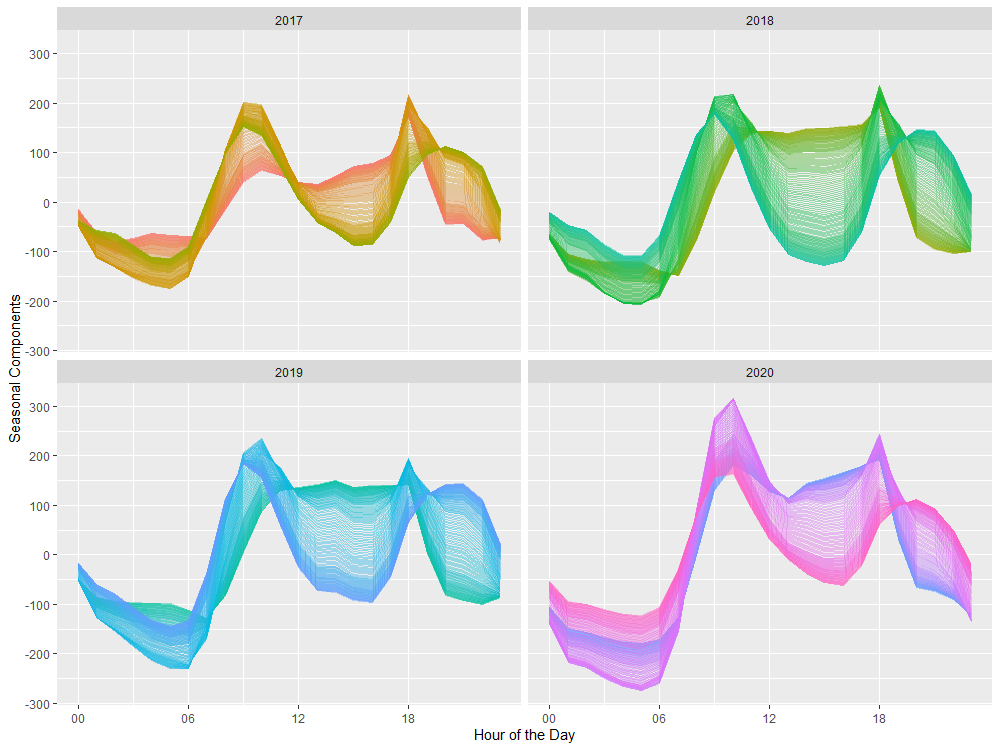
\includegraphics[width=.55\textwidth,height=.55\textheight,keepaspectratio]{images/daily_seasonal.png}
  \caption{The presence of multiple seasonal cycles%
    \footnote{%
     \tiny{Github repo: https://github.com/kasungayan/Meldatathon2020} 
    }%
  }
\end{figure}

\end{frame}

\begin{frame}{Model Development (MD)}
\protect\hypertarget{model-development-md}{}

\begin{itemize}
\tightlist
\item
  Model parameter estimation, Hyper-parameter tuning. \vspace{2mm}

  \begin{figure}
  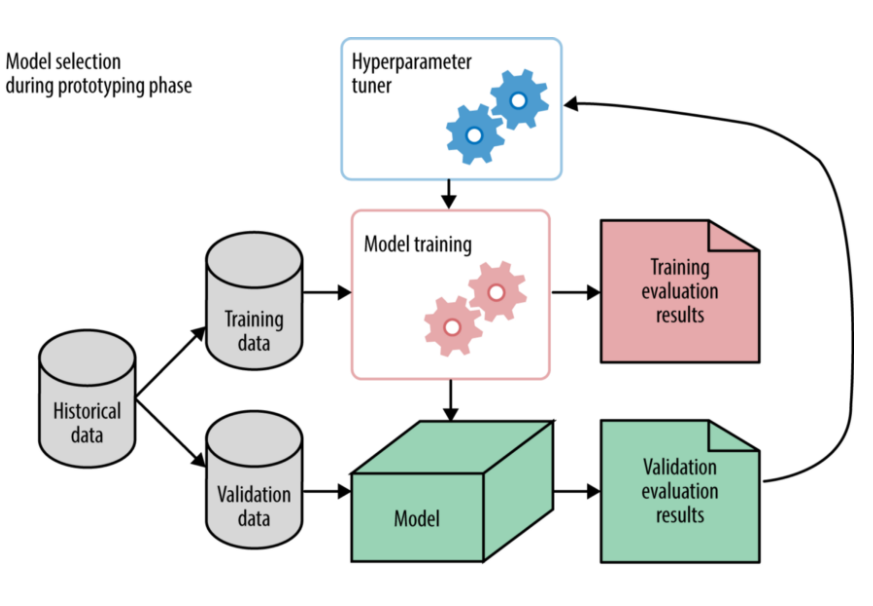
\includegraphics[width=.6\textwidth,height=.6\textheight,keepaspectratio]{images/model_validation.PNG}
  \caption{Model Training and Validation%
    \footnote{%
     \tiny{Image source: https://towardsdatascience.com/5-steps-of-a-data-science-project-lifecycle-26c50372b492} 
    }%
  }
  \end{figure}
\end{itemize}

\end{frame}

\begin{frame}{Model Development Techniques}
\protect\hypertarget{model-development-techniques}{}

\begin{itemize}
\tightlist
\item
  \textbf{Supervised Learning} or \textbf{Unsupervised Learning}
  \vspace{2mm}

  \begin{itemize}
      \item Regression: Linear-regression, Support Vector Machine (SVM), Lasso-Regression
      \item Classification: Naive Bayes, Random Forest, K-Nearest Neighbors
      \item Clustering: K-Means, Fuzzy C-Means, Self Organising Maps (SOM) 
    \end{itemize}
  \vspace{2mm}
\item
  Neural Networks: Multilayer Perceptron (\textbf{MLP}), Recurrent
  Neural Network (\textbf{RNN}), Convolutional Neural Network
  (\textbf{CNN}) \vspace{2mm}
\item
  Different applications: \textbf{Spam Detection}, \textbf{Market
  Segmentation}, \textbf{Image Classification}, \textbf{Time Series
  Forecasting}, \textbf{Language Translation}, \textbf{Voice
  Recognition}
\end{itemize}

\end{frame}

\begin{frame}[fragile]{Naive Bayes classifier}
\protect\hypertarget{naive-bayes-classifier}{}

\tiny

\begin{Shaded}
\begin{Highlighting}[]
\KeywordTok{library}\NormalTok{(mlbench) }\CommentTok{# multiple benchmark datasets for different machine learning tasks.}
\KeywordTok{library}\NormalTok{(caret) }\CommentTok{# multiple inbuilt regression and classification algorithms.}
\KeywordTok{library}\NormalTok{(rsample) }\CommentTok{# data splitting.}
\KeywordTok{library}\NormalTok{(dplyr)}

\KeywordTok{data}\NormalTok{(BreastCancer)}
\KeywordTok{set.seed}\NormalTok{(}\DecValTok{1234}\NormalTok{)}

\CommentTok{# Splitting the data into train and test sets.}
\NormalTok{df_BreastCancer_split <-}\StringTok{ }\KeywordTok{initial_split}\NormalTok{(BreastCancer, }\DataTypeTok{prop =} \FloatTok{.7}\NormalTok{)}
\CommentTok{# Similar splitting using caTools}
\CommentTok{# df_BreastCancer_split <- sample.split(BreastCancer,SplitRatio = 0.7)}

\NormalTok{df_BreastCancer_train <-}\StringTok{ }\KeywordTok{training}\NormalTok{(df_BreastCancer_split)}
\NormalTok{df_BreastCancer_test  <-}\StringTok{ }\KeywordTok{testing}\NormalTok{(df_BreastCancer_split)}

\CommentTok{# Checking for class distribution.}
\KeywordTok{table}\NormalTok{(df_BreastCancer_train}\OperatorTok{$}\NormalTok{Class) }\OperatorTok\StringTok{ }\KeywordTok{prop.table}\NormalTok{()}
\end{Highlighting}
\end{Shaded}

\begin{verbatim}
## 
##    benign malignant 
## 0.6571429 0.3428571
\end{verbatim}

\begin{Shaded}
\begin{Highlighting}[]
\KeywordTok{table}\NormalTok{(df_BreastCancer_test}\OperatorTok{$}\NormalTok{Class) }\OperatorTok\StringTok{ }\KeywordTok{prop.table}\NormalTok{()}
\end{Highlighting}
\end{Shaded}

\begin{verbatim}
## 
##    benign malignant 
## 0.6507177 0.3492823
\end{verbatim}

\normalsize

\end{frame}

\begin{frame}[fragile]{Naive Bayes classifier Cont.}
\protect\hypertarget{naive-bayes-classifier-cont.}{}

\tiny

\begin{Shaded}
\begin{Highlighting}[]
\CommentTok{# create feature and class attributes.}
\NormalTok{features <-}\StringTok{ }\KeywordTok{setdiff}\NormalTok{(}\KeywordTok{names}\NormalTok{(df_BreastCancer_train), }\StringTok{"Class"}\NormalTok{)}
\NormalTok{train_features <-}\StringTok{ }\NormalTok{df_BreastCancer_train[, features]}
\NormalTok{train_class <-}\StringTok{ }\NormalTok{df_BreastCancer_train}\OperatorTok{$}\NormalTok{Class}

\CommentTok{# Define a 10-fold cross validation procedure.}
\NormalTok{train_control <-}\StringTok{ }\KeywordTok{trainControl}\NormalTok{(}\DataTypeTok{method =} \StringTok{"cv"}\NormalTok{, }\DataTypeTok{number =} \DecValTok{10}\NormalTok{)}

\CommentTok{# train the naive bayes model}
\NormalTok{model_nb1 <-}\StringTok{ }\KeywordTok{train}\NormalTok{(}\DataTypeTok{x =}\NormalTok{ train_features, }\DataTypeTok{y =}\NormalTok{ train_class, }\DataTypeTok{method =} \StringTok{"nb"}\NormalTok{, }\DataTypeTok{trControl =}\NormalTok{ train_control)}
\CommentTok{#Show the confusion matrix.}
\KeywordTok{confusionMatrix}\NormalTok{(model_nb1)}
\end{Highlighting}
\end{Shaded}

\begin{verbatim}
## Cross-Validated (10 fold) Confusion Matrix 
## 
## (entries are percentual average cell counts across resamples)
##  
##            Reference
## Prediction  benign malignant
##   benign      63.5       0.4
##   malignant    2.2      33.9
##                             
##  Accuracy (average) : 0.9735
\end{verbatim}

\normalsize

\end{frame}

\begin{frame}[fragile]{Naive Bayes classifier Cont.}
\protect\hypertarget{naive-bayes-classifier-cont.-1}{}

\tiny

\begin{Shaded}
\begin{Highlighting}[]
\CommentTok{# hyper-parameter grid}
\NormalTok{hyper_search_grid <-}\StringTok{ }\KeywordTok{expand.grid}\NormalTok{(}\DataTypeTok{usekernel =} \KeywordTok{c}\NormalTok{(}\OtherTok{TRUE}\NormalTok{, }\OtherTok{FALSE}\NormalTok{), }\DataTypeTok{fL =} \DecValTok{0}\OperatorTok{:}\DecValTok{5}\NormalTok{, }\DataTypeTok{adjust =} \KeywordTok{seq}\NormalTok{(}\DecValTok{0}\NormalTok{, }\DecValTok{5}\NormalTok{, }\DataTypeTok{by =} \DecValTok{1}\NormalTok{))}

\CommentTok{# train the naive bayes model using a hyper-parameter grid.}
\NormalTok{model_nb2 <-}\StringTok{ }\KeywordTok{train}\NormalTok{(}\DataTypeTok{x =}\NormalTok{ train_features, }\DataTypeTok{y =}\NormalTok{ train_class, }\DataTypeTok{method =} \StringTok{"nb"}\NormalTok{, }
                   \DataTypeTok{trControl =}\NormalTok{ train_control, }\DataTypeTok{tuneGrid =}\NormalTok{ hyper_search_grid)}

\CommentTok{# Printing best models.}
\CommentTok{# model_nb2$results %>% }
\CommentTok{#  arrange(desc(Accuracy)) %>% head(4)}

\CommentTok{# results for best model}
\KeywordTok{confusionMatrix}\NormalTok{(model_nb2)}
\end{Highlighting}
\end{Shaded}

\begin{verbatim}
## Cross-Validated (10 fold) Confusion Matrix 
## 
## (entries are percentual average cell counts across resamples)
##  
##            Reference
## Prediction  benign malignant
##   benign      63.5       0.8
##   malignant    2.2      33.5
##                             
##  Accuracy (average) : 0.9694
\end{verbatim}

\normalsize

\end{frame}

\begin{frame}[fragile]{Naive Bayes results on the testset}
\protect\hypertarget{naive-bayes-results-on-the-testset}{}

\tiny

\begin{Shaded}
\begin{Highlighting}[]
\CommentTok{# Applying the best model to unseen (test) dataset.}
\NormalTok{prediction_test <-}\StringTok{ }\KeywordTok{predict}\NormalTok{(model_nb2, }\DataTypeTok{newdata =}\NormalTok{ df_BreastCancer_test)}
\CommentTok{# Printing the confusing matrix on the test set.}
\KeywordTok{confusionMatrix}\NormalTok{(prediction_test, df_BreastCancer_test}\OperatorTok{$}\NormalTok{Class)}
\end{Highlighting}
\end{Shaded}

\begin{verbatim}
## Confusion Matrix and Statistics
## 
##            Reference
## Prediction  benign malignant
##   benign       132         1
##   malignant      4        72
##                                           
##                Accuracy : 0.9761          
##                  95% CI : (0.9451, 0.9922)
##     No Information Rate : 0.6507          
##     P-Value [Acc > NIR] : <2e-16          
##                                           
##                   Kappa : 0.9479          
##                                           
##  Mcnemar's Test P-Value : 0.3711          
##                                           
##             Sensitivity : 0.9706          
##             Specificity : 0.9863          
##          Pos Pred Value : 0.9925          
##          Neg Pred Value : 0.9474          
##              Prevalence : 0.6507          
##          Detection Rate : 0.6316          
##    Detection Prevalence : 0.6364          
##       Balanced Accuracy : 0.9784          
##                                           
##        'Positive' Class : benign          
## 
\end{verbatim}

\normalsize

\end{frame}

\begin{frame}[fragile]{Generating the ROC curve}
\protect\hypertarget{generating-the-roc-curve}{}

\tiny

\begin{Shaded}
\begin{Highlighting}[]
\KeywordTok{library}\NormalTok{(caTools) }\CommentTok{#to generate ROC curves}

\NormalTok{prob_results <-}\StringTok{ }\KeywordTok{predict}\NormalTok{(model_nb2, df_BreastCancer_test, }\DataTypeTok{type =} \StringTok{"prob"}\NormalTok{)}

\CommentTok{# Generating the ROC curve for the test set.}
\NormalTok{caTools}\OperatorTok{::}\KeywordTok{colAUC}\NormalTok{(prob_results, df_BreastCancer_test[[}\StringTok{"Class"}\NormalTok{]], }\DataTypeTok{plotROC =} \OtherTok{TRUE}\NormalTok{)}
\end{Highlighting}
\end{Shaded}

\begin{center}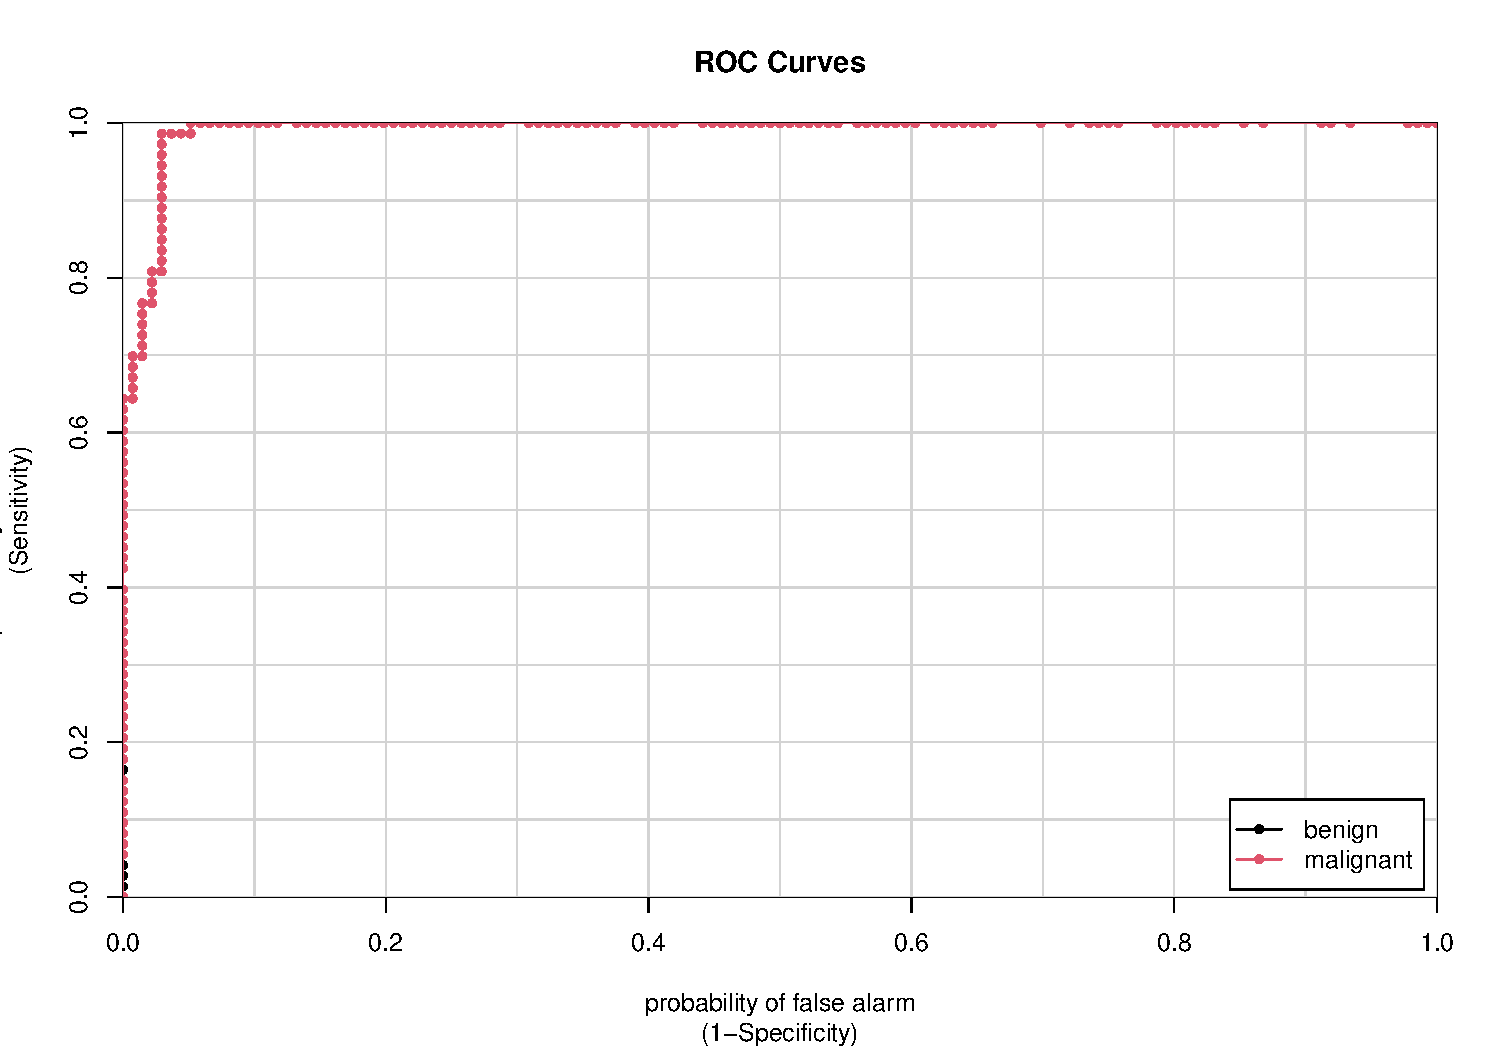
\includegraphics[width=0.7\linewidth,height=0.6\textheight]{figs/unnamed-chunk-9} \end{center}

\begin{verbatim}
##                         benign malignant
## benign vs. malignant 0.9917405 0.9917405
\end{verbatim}

\normalsize

\end{frame}

\begin{frame}[fragile]{Decision tree}
\protect\hypertarget{decision-tree}{}

\tiny

\begin{Shaded}
\begin{Highlighting}[]
\KeywordTok{library}\NormalTok{(caret)}
\KeywordTok{library}\NormalTok{(rpart)}

\KeywordTok{set.seed}\NormalTok{(}\DecValTok{1234}\NormalTok{)}

\CommentTok{# Remove incomplete records.}
\NormalTok{df_BreastCancer_train <-}\StringTok{ }\NormalTok{df_BreastCancer_train[}\KeywordTok{complete.cases}\NormalTok{(df_BreastCancer_train), ]}

\CommentTok{# Define a 10-fold cross validation procedure.}
\NormalTok{train_control <-}\StringTok{ }\KeywordTok{trainControl}\NormalTok{(}\DataTypeTok{method =} \StringTok{"cv"}\NormalTok{, }\DataTypeTok{number =} \DecValTok{10}\NormalTok{)}

\CommentTok{# train the naive bayes model.}
\NormalTok{model_dt <-}\StringTok{ }\KeywordTok{train}\NormalTok{(Class }\OperatorTok{~}\StringTok{ }\NormalTok{., }\DataTypeTok{data=}\NormalTok{df_BreastCancer_train, }\DataTypeTok{method =} \StringTok{"rpart"}\NormalTok{, }\DataTypeTok{trControl =}\NormalTok{ train_control)}
\CommentTok{#Show the confusion matrix.}
\KeywordTok{confusionMatrix}\NormalTok{(model_dt)}
\end{Highlighting}
\end{Shaded}

\begin{verbatim}
## Cross-Validated (10 fold) Confusion Matrix 
## 
## (entries are percentual average cell counts across resamples)
##  
##            Reference
## Prediction  benign malignant
##   benign      62.2       3.3
##   malignant    3.1      31.3
##                             
##  Accuracy (average) : 0.9357
\end{verbatim}

\normalsize

\end{frame}

\begin{frame}[fragile]{Visualising the decision tree}
\protect\hypertarget{visualising-the-decision-tree}{}

\tiny

\begin{Shaded}
\begin{Highlighting}[]
\KeywordTok{library}\NormalTok{(rattle)}
\KeywordTok{set.seed}\NormalTok{(}\DecValTok{1234}\NormalTok{)}
\CommentTok{# Generating the decision tree.}
\CommentTok{# You can also separately use the rpart and rpart.plot to reproduce this.}

\KeywordTok{fancyRpartPlot}\NormalTok{(model_dt}\OperatorTok{$}\NormalTok{finalModel)}
\end{Highlighting}
\end{Shaded}

\begin{center}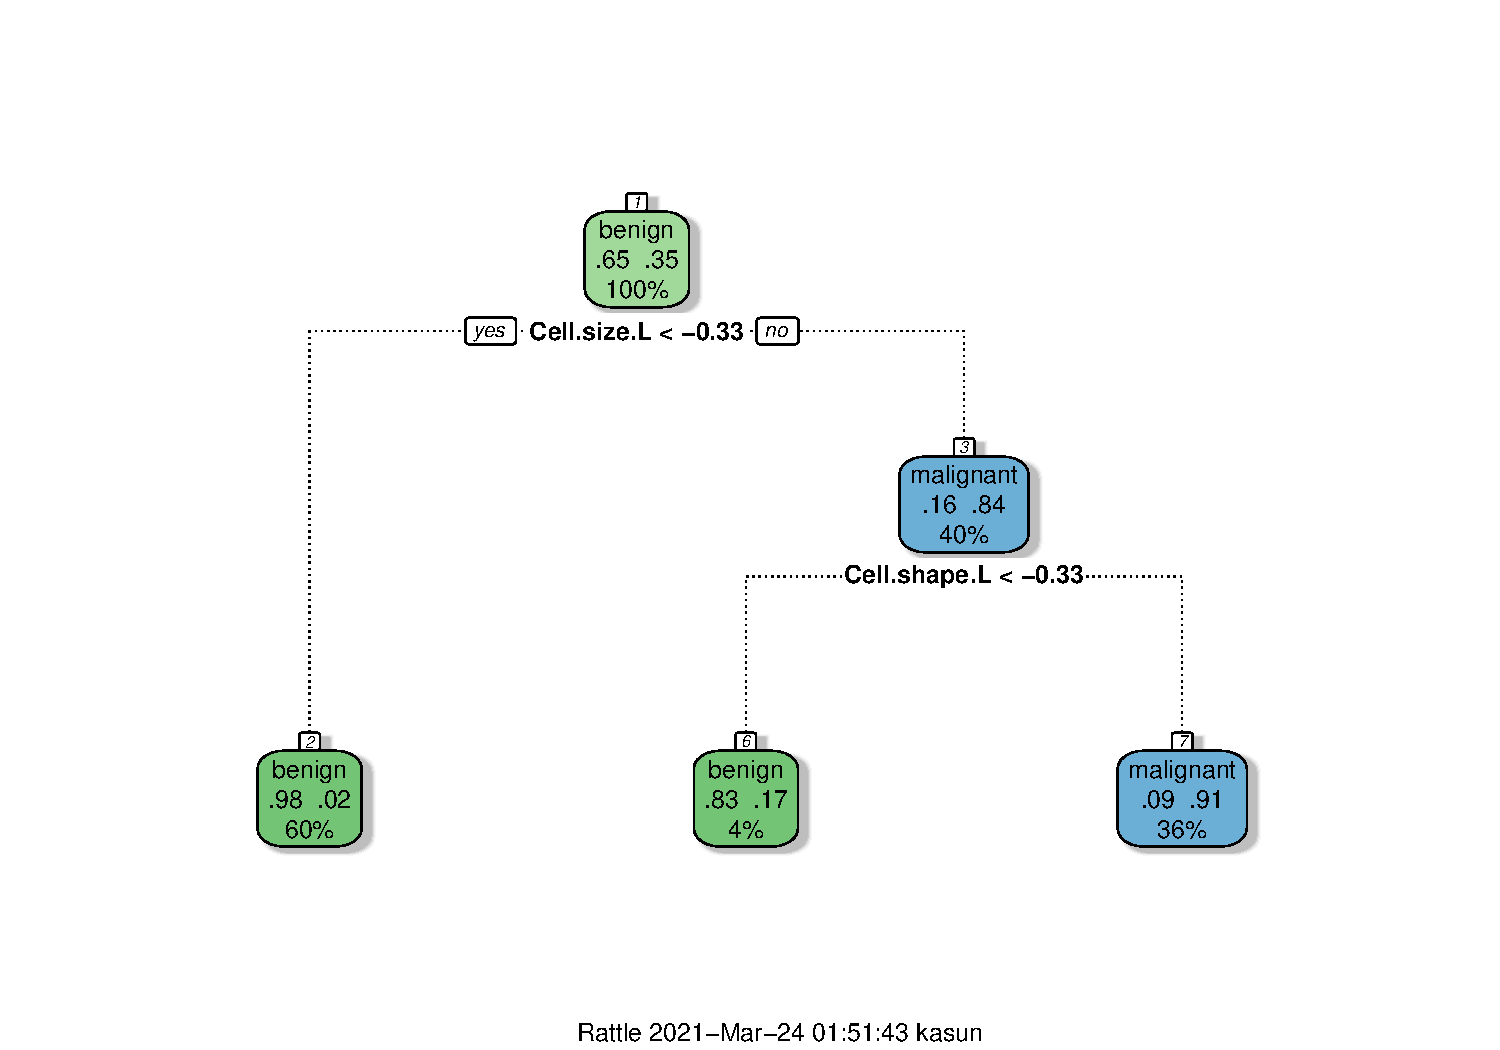
\includegraphics[width=0.8\linewidth,height=0.7\textheight]{figs/unnamed-chunk-11} \end{center}

\normalsize

\end{frame}

\begin{frame}[fragile]{Regression using \texttt{\{caret\}}}
\protect\hypertarget{regression-using}{}

\tiny

\begin{Shaded}
\begin{Highlighting}[]
\KeywordTok{data}\NormalTok{(diamonds)}
\KeywordTok{set.seed}\NormalTok{(}\DecValTok{1234}\NormalTok{)}

\CommentTok{# Data splitting.}
\NormalTok{data_split <-}\StringTok{ }\KeywordTok{initial_split}\NormalTok{(diamonds, }\DataTypeTok{prop =} \FloatTok{.7}\NormalTok{)}
\NormalTok{train <-}\StringTok{ }\KeywordTok{training}\NormalTok{(data_split)}
\NormalTok{test  <-}\StringTok{ }\KeywordTok{testing}\NormalTok{(data_split)}

\CommentTok{# Linear regression model training.}
\NormalTok{model <-}\StringTok{ }\KeywordTok{train}\NormalTok{(price }\OperatorTok{~}\StringTok{ }\NormalTok{., train, }\DataTypeTok{method =} \StringTok{"lm"}\NormalTok{,}\DataTypeTok{trControl =} \KeywordTok{trainControl}\NormalTok{(}\DataTypeTok{method =} \StringTok{"cv"}\NormalTok{,}
                                        \DataTypeTok{number =} \DecValTok{10}\NormalTok{))}
\KeywordTok{print}\NormalTok{(model)}
\end{Highlighting}
\end{Shaded}

\begin{verbatim}
## Linear Regression 
## 
## 37758 samples
##     9 predictor
## 
## No pre-processing
## Resampling: Cross-Validated (10 fold) 
## Summary of sample sizes: 33982, 33982, 33983, 33982, 33982, 33981, ... 
## Resampling results:
## 
##   RMSE      Rsquared   MAE     
##   1126.445  0.9204881  742.5132
## 
## Tuning parameter 'intercept' was held constant at a value of TRUE
\end{verbatim}

\normalsize

\end{frame}

\begin{frame}[fragile]{Regression using \texttt{\{glmnet\}}}
\protect\hypertarget{regression-using-1}{}

\tiny

\begin{Shaded}
\begin{Highlighting}[]
\KeywordTok{library}\NormalTok{(glmnet)}
\KeywordTok{library}\NormalTok{(dplyr)}

\KeywordTok{data}\NormalTok{(diamonds)}
\KeywordTok{set.seed}\NormalTok{(}\DecValTok{1234}\NormalTok{)}
\CommentTok{# Defining the feature variables.}
\NormalTok{x <-}\StringTok{ }\KeywordTok{model.matrix}\NormalTok{(price}\OperatorTok{~}\NormalTok{., train)[,}\OperatorTok{-}\DecValTok{1}\NormalTok{]}
\CommentTok{# Defining the class variable.}
\NormalTok{y <-}\StringTok{ }\NormalTok{train}\OperatorTok{$}\NormalTok{price}

\CommentTok{# Use cross validation to determine the optimal lambda.}
\NormalTok{cv <-}\StringTok{ }\KeywordTok{cv.glmnet}\NormalTok{(x, y, }\DataTypeTok{alpha =} \DecValTok{1}\NormalTok{)}
\CommentTok{# Fit the final model (lasso regression) on the training data}
\NormalTok{best_model <-}\StringTok{ }\KeywordTok{glmnet}\NormalTok{(x, y, }\DataTypeTok{alpha =} \DecValTok{1}\NormalTok{, }\DataTypeTok{lambda =}\NormalTok{ cv}\OperatorTok{$}\NormalTok{lambda.min)}

\CommentTok{# Evaluating the model on the test data.}
\NormalTok{x.test <-}\StringTok{ }\KeywordTok{model.matrix}\NormalTok{(price}\OperatorTok{~}\StringTok{ }\NormalTok{., test)[,}\OperatorTok{-}\DecValTok{1}\NormalTok{]}
\NormalTok{price_predictions <-}\StringTok{ }\NormalTok{best_model }\OperatorTok\StringTok{ }\KeywordTok{predict}\NormalTok{(x.test) }\OperatorTok\StringTok{ }\KeywordTok{as.numeric}\NormalTok{()}
\NormalTok{price_predictions[price_predictions }\OperatorTok{<}\StringTok{ }\DecValTok{0}\NormalTok{] <-}\StringTok{ }\DecValTok{0}

\CommentTok{# Model performance summary.}
\KeywordTok{data.frame}\NormalTok{(}
  \DataTypeTok{RMSE =} \KeywordTok{RMSE}\NormalTok{(price_predictions, test}\OperatorTok{$}\NormalTok{price),}
  \DataTypeTok{Rsquare =} \KeywordTok{R2}\NormalTok{(price_predictions, test}\OperatorTok{$}\NormalTok{price)}
\NormalTok{)}
\end{Highlighting}
\end{Shaded}

\begin{verbatim}
##       RMSE   Rsquare
## 1 1088.945 0.9254219
\end{verbatim}

\normalsize

\end{frame}

\begin{frame}[fragile]{Regression using \texttt{\{glmnet\}}}
\protect\hypertarget{regression-using-2}{}

\tiny

\begin{Shaded}
\begin{Highlighting}[]
\KeywordTok{library}\NormalTok{(glmnet)}
\KeywordTok{library}\NormalTok{(dplyr)}

\KeywordTok{data}\NormalTok{(diamonds)}
\KeywordTok{set.seed}\NormalTok{(}\DecValTok{1234}\NormalTok{)}
\CommentTok{# Defining the feature variables.}
\NormalTok{x <-}\StringTok{ }\KeywordTok{model.matrix}\NormalTok{(price}\OperatorTok{~}\NormalTok{., train)[,}\OperatorTok{-}\DecValTok{1}\NormalTok{]}
\CommentTok{# Defining the class variable.}
\NormalTok{y <-}\StringTok{ }\NormalTok{train}\OperatorTok{$}\NormalTok{price}

\CommentTok{# Use cross validation to determine the optimal lambda.}
\NormalTok{cv <-}\StringTok{ }\KeywordTok{cv.glmnet}\NormalTok{(x, y, }\DataTypeTok{alpha =} \DecValTok{1}\NormalTok{)}
\CommentTok{# Fit the final model (lasso regression) on the training data}
\NormalTok{best_model <-}\StringTok{ }\KeywordTok{glmnet}\NormalTok{(x, y, }\DataTypeTok{alpha =} \DecValTok{1}\NormalTok{, }\DataTypeTok{lambda =}\NormalTok{ cv}\OperatorTok{$}\NormalTok{lambda.min)}

\CommentTok{# Evaluating the model on the test data.}
\NormalTok{x.test <-}\StringTok{ }\KeywordTok{model.matrix}\NormalTok{(price}\OperatorTok{~}\StringTok{ }\NormalTok{., test)[,}\OperatorTok{-}\DecValTok{1}\NormalTok{]}
\NormalTok{price_predictions <-}\StringTok{ }\NormalTok{best_model }\OperatorTok\StringTok{ }\KeywordTok{predict}\NormalTok{(x.test) }\OperatorTok\StringTok{ }\KeywordTok{as.numeric}\NormalTok{()}
\NormalTok{price_predictions[price_predictions }\OperatorTok{<}\StringTok{ }\DecValTok{0}\NormalTok{] <-}\StringTok{ }\DecValTok{0}

\CommentTok{# Model performance summary.}
\KeywordTok{data.frame}\NormalTok{(}
  \DataTypeTok{RMSE =} \KeywordTok{RMSE}\NormalTok{(price_predictions, test}\OperatorTok{$}\NormalTok{price),}
  \DataTypeTok{Rsquare =} \KeywordTok{R2}\NormalTok{(price_predictions, test}\OperatorTok{$}\NormalTok{price)}
\NormalTok{)}
\end{Highlighting}
\end{Shaded}

\begin{verbatim}
##       RMSE   Rsquare
## 1 1088.945 0.9254219
\end{verbatim}

\normalsize

\end{frame}

\begin{frame}{Unsupervised Learning}
\protect\hypertarget{unsupervised-learning}{}

\begin{itemize}
\tightlist
\item
  Learning patterns from unlabbled data. \vspace{2mm}
\item
  Clustering ? \vspace{2mm}

  \begin{itemize}
      \item K means: Computationally efficient, \textbf{Optimal K ?, Outliers?}
      \item Elbow and Silhouette methods to determine the optimal K
      \item \textbf{DBSCAN}: No restrictions on the cluster shapes
      \item Feature are categorical ? \textbf{Partitioning Around Medoids (PAM)}
      \item Hierarchical clustering: \textbf{cluster dendrogram}
    \end{itemize}
  \vspace{2mm}
\item
  Auto-Encoders ?
\end{itemize}

\end{frame}

\begin{frame}[fragile]{Kmeans clustering}
\protect\hypertarget{kmeans-clustering}{}

\tiny

\begin{Shaded}
\begin{Highlighting}[]
\KeywordTok{library}\NormalTok{(factoextra)}

\KeywordTok{set.seed}\NormalTok{(}\DecValTok{1234}\NormalTok{)}

\CommentTok{# Removing the categorical class.}
\NormalTok{df <-}\StringTok{ }\NormalTok{iris[, }\DecValTok{-5}\NormalTok{]}
\CommentTok{# Applying kmeans algorithm with k = 3.}
\NormalTok{cluster_output <-}\StringTok{ }\KeywordTok{kmeans}\NormalTok{(df, }\DataTypeTok{centers =} \DecValTok{3}\NormalTok{, }\DataTypeTok{nstart =} \DecValTok{25}\NormalTok{)}
\CommentTok{# Illustrating the cluster distribution.}
\KeywordTok{fviz_cluster}\NormalTok{(cluster_output, }\DataTypeTok{data =}\NormalTok{ df)}
\end{Highlighting}
\end{Shaded}

\begin{center}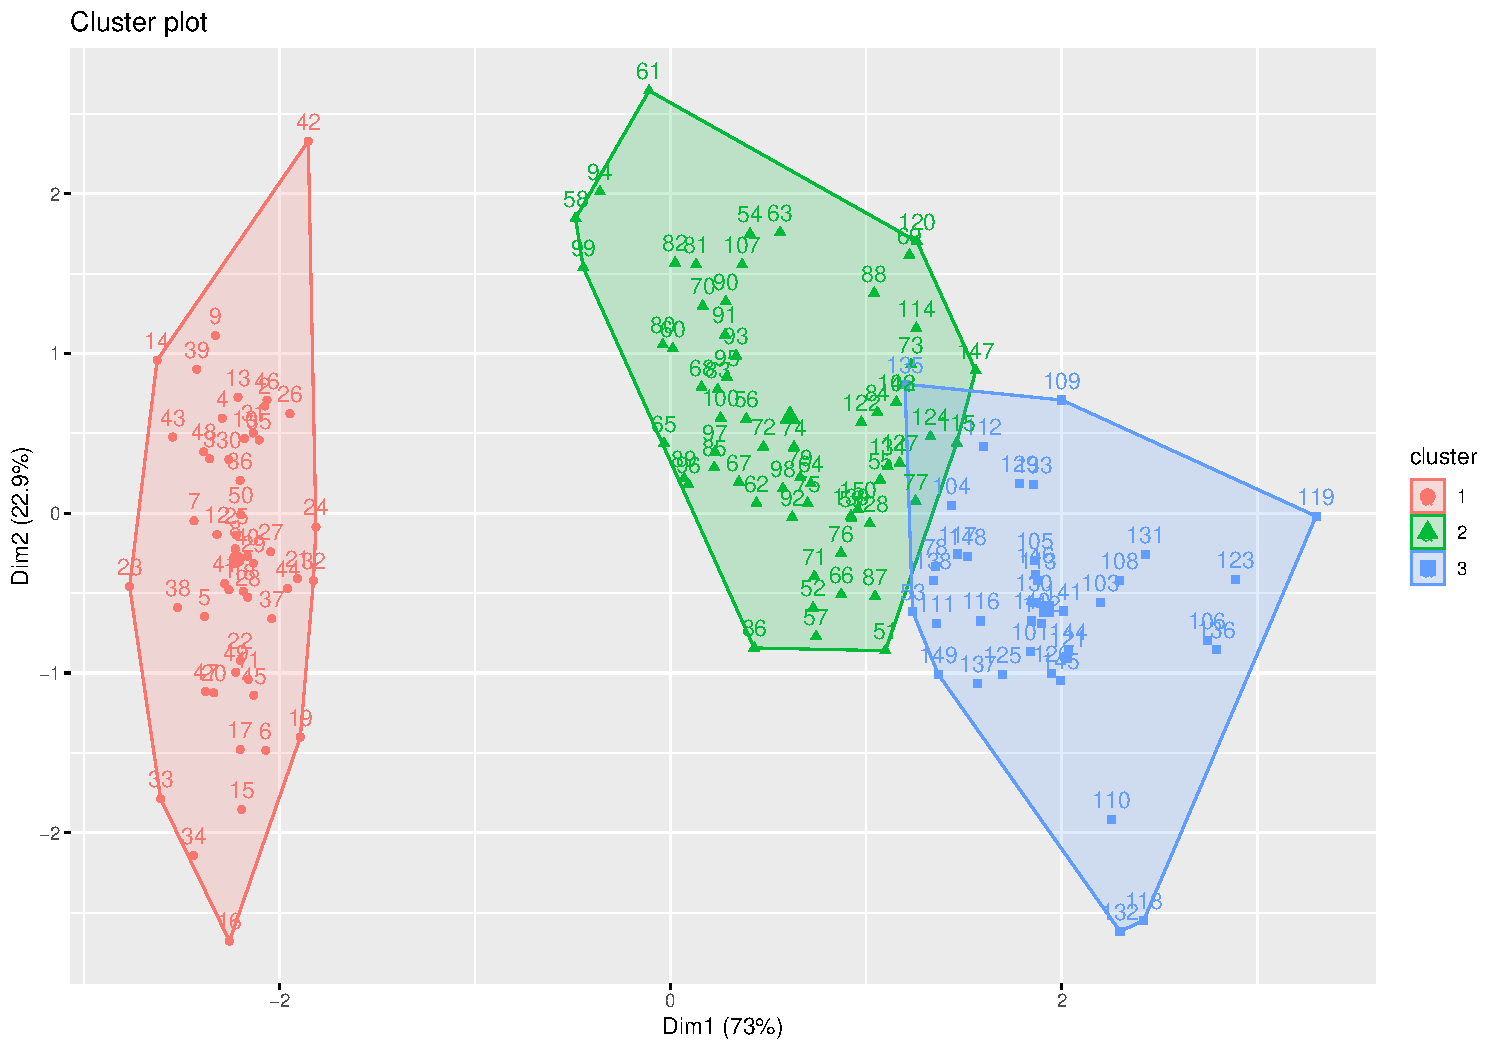
\includegraphics[width=0.6\linewidth,height=0.5\textheight]{figs/unnamed-chunk-15} \end{center}

\normalsize

\end{frame}

\begin{frame}[fragile]{Optimal K}
\protect\hypertarget{optimal-k}{}

\tiny

\begin{Shaded}
\begin{Highlighting}[]
\KeywordTok{library}\NormalTok{(gridExtra)}

\KeywordTok{set.seed}\NormalTok{(}\DecValTok{1234}\NormalTok{)}
\CommentTok{# Different methods to determine the optimal K.}
\NormalTok{elbow <-}\StringTok{ }\KeywordTok{fviz_nbclust}\NormalTok{(df, kmeans, }\DataTypeTok{method =} \StringTok{"wss"}\NormalTok{)}
\NormalTok{silhouette <-}\StringTok{ }\KeywordTok{fviz_nbclust}\NormalTok{(df, kmeans, }\DataTypeTok{method =} \StringTok{"silhouette"}\NormalTok{)}

\KeywordTok{grid.arrange}\NormalTok{(elbow, silhouette, }\DataTypeTok{nrow =} \DecValTok{1}\NormalTok{)}
\end{Highlighting}
\end{Shaded}

\begin{center}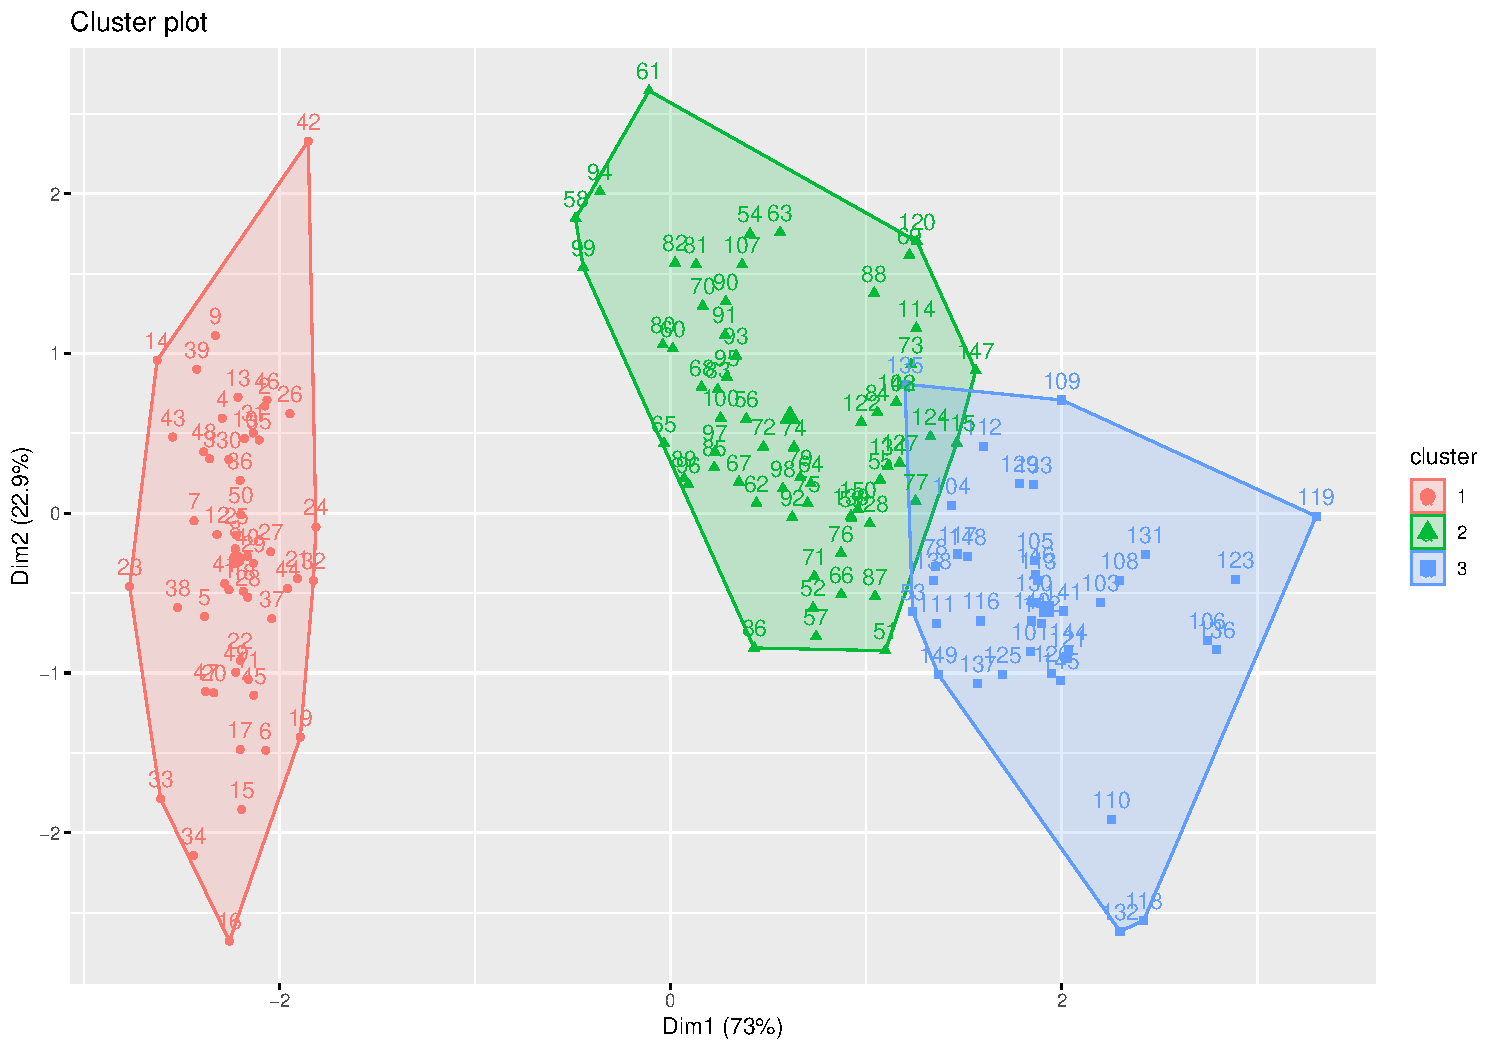
\includegraphics[width=0.7\linewidth,height=0.6\textheight]{figs/unnamed-chunk-16} \end{center}

\normalsize

\end{frame}

\begin{frame}[fragile]{Clustering using DBSCAN}
\protect\hypertarget{clustering-using-dbscan}{}

\tiny

\begin{Shaded}
\begin{Highlighting}[]
\KeywordTok{library}\NormalTok{(factoextra)}
\KeywordTok{library}\NormalTok{(fpc)}

\KeywordTok{set.seed}\NormalTok{(}\DecValTok{1234}\NormalTok{)}
\NormalTok{df <-}\StringTok{ }\NormalTok{iris[, }\DecValTok{-5}\NormalTok{]}

\CommentTok{# Using DBSCAN algorithm without setting the K.}
\NormalTok{db_output <-}\StringTok{ }\NormalTok{fpc}\OperatorTok{::}\KeywordTok{dbscan}\NormalTok{(df, }\DataTypeTok{eps =} \FloatTok{0.95}\NormalTok{, }\DataTypeTok{MinPts =} \DecValTok{5}\NormalTok{)}
\KeywordTok{fviz_cluster}\NormalTok{(db_output, df, }\DataTypeTok{stand =} \OtherTok{FALSE}\NormalTok{, }\DataTypeTok{frame =} \OtherTok{FALSE}\NormalTok{, }\DataTypeTok{geom =} \StringTok{"point"}\NormalTok{)}
\end{Highlighting}
\end{Shaded}

\begin{center}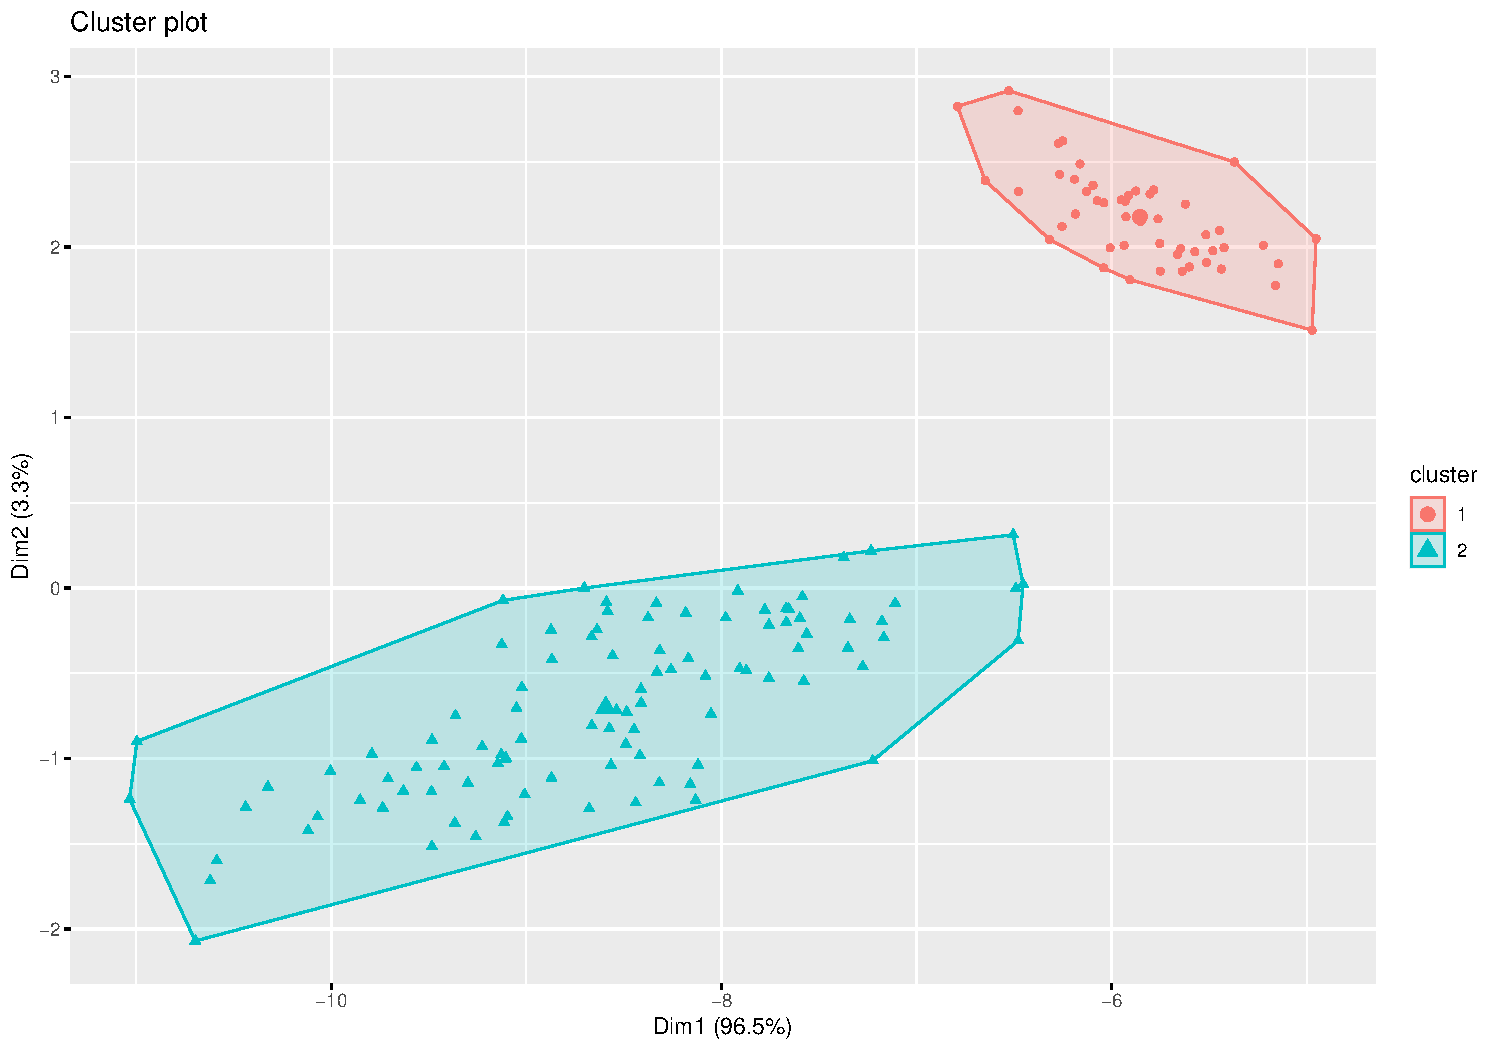
\includegraphics[width=0.7\linewidth,height=0.6\textheight]{figs/unnamed-chunk-17} \end{center}

\normalsize

\end{frame}

\begin{frame}{Neural Networks}
\protect\hypertarget{neural-networks}{}

\begin{itemize}
\tightlist
\item
  Strong computational systems that mimic human brain.
\item
  Hold the universal approximation property.
\item
  Backpropagation algorithm for training.
\item
  State-of-the-art for many prediction/classification applications.
\item
  Different variants of neural networks.

  \begin{itemize}
      \item Multi-Layer Perceptrons (MLP): \texttt{\{nnet,neuralnet\}}
      \item Recurrent Neural Networks (RNN): \texttt{\{rnn,RSNNS\}}
      \item Convolutional neural networks (CNNs)
    \end{itemize}
\item
  \textbf{Tensorflow, Keras, Torch} APIs in R
\end{itemize}

\end{frame}

\begin{frame}[fragile]{Feedforward Neural Networks using
\texttt{\{nnet\}}}
\protect\hypertarget{feedforward-neural-networks-using}{}

\tiny

\begin{Shaded}
\begin{Highlighting}[]
\KeywordTok{library}\NormalTok{(caret)}

\KeywordTok{data}\NormalTok{(diamonds)}
\KeywordTok{set.seed}\NormalTok{(}\DecValTok{1234}\NormalTok{)}

\CommentTok{# Preprocessing.}
\CommentTok{# Use model.matrix for categorical variables (one-hot encoding)}
\NormalTok{df_diamonds <-}\StringTok{ }\NormalTok{diamonds[, }\KeywordTok{c}\NormalTok{(}\OperatorTok{-}\DecValTok{2}\NormalTok{, }\DecValTok{-3}\NormalTok{, }\DecValTok{-4}\NormalTok{)]}

\CommentTok{# Data splitting.}
\NormalTok{data_split <-}\StringTok{ }\KeywordTok{initial_split}\NormalTok{(df_diamonds, }\DataTypeTok{prop =} \FloatTok{.7}\NormalTok{)}
\NormalTok{train <-}\StringTok{ }\KeywordTok{training}\NormalTok{(data_split)}
\NormalTok{test  <-}\StringTok{ }\KeywordTok{testing}\NormalTok{(data_split)}

\CommentTok{# You can directly use the nnet function from the nnet packaage}
\CommentTok{# mlp_fit <- nnet(price ~ ., train, size = 2, rang = 0.1, decay = 5e-4, maxit = 200)}

\CommentTok{# You can use the nnet as the method in the caret function.}
\NormalTok{mlp_fit <-}\StringTok{ }\KeywordTok{train}\NormalTok{(price }\OperatorTok{~}\StringTok{ }\NormalTok{., train, }\DataTypeTok{method =} \StringTok{"nnet"}\NormalTok{,}\DataTypeTok{trControl =} \KeywordTok{trainControl}\NormalTok{(}\DataTypeTok{method =} \StringTok{"cv"}\NormalTok{,}
                                        \DataTypeTok{number =} \DecValTok{10}\NormalTok{))}
\CommentTok{#print(mlp_fit)}
\end{Highlighting}
\end{Shaded}

\normalsize

\end{frame}

\begin{frame}[fragile]{Deep Neural Netowrks using \texttt{\{keras\}}}
\protect\hypertarget{deep-neural-netowrks-using}{}

\tiny

\begin{Shaded}
\begin{Highlighting}[]
\KeywordTok{library}\NormalTok{(keras)}
\KeywordTok{library}\NormalTok{(rsample)}
\KeywordTok{library}\NormalTok{(ggplot2)}
\KeywordTok{library}\NormalTok{(dplyr)}

\KeywordTok{data}\NormalTok{(diamonds)}
\KeywordTok{set.seed}\NormalTok{(}\DecValTok{1234}\NormalTok{)}

\CommentTok{# The initial preprocessing.}
\CommentTok{# Use model.matrix for categorical variables (one-hot encoding)}
\NormalTok{df_diamonds <-}\StringTok{ }\NormalTok{diamonds[, }\KeywordTok{c}\NormalTok{(}\OperatorTok{-}\DecValTok{2}\NormalTok{, }\DecValTok{-3}\NormalTok{, }\DecValTok{-4}\NormalTok{)]}

\CommentTok{# Data splitting.}
\NormalTok{data_split <-}\StringTok{ }\KeywordTok{initial_split}\NormalTok{(df_diamonds, }\DataTypeTok{prop =} \FloatTok{.7}\NormalTok{)}
\NormalTok{train <-}\StringTok{ }\KeywordTok{training}\NormalTok{(data_split)}
\NormalTok{test  <-}\StringTok{ }\KeywordTok{testing}\NormalTok{(data_split)}

\NormalTok{features <-}\StringTok{ }\KeywordTok{setdiff}\NormalTok{(}\KeywordTok{names}\NormalTok{(train), }\StringTok{"price"}\NormalTok{)}
\NormalTok{train_features <-}\StringTok{ }\NormalTok{train[, features]}
\NormalTok{train_class <-}\StringTok{ }\NormalTok{train}\OperatorTok{$}\NormalTok{price}
\end{Highlighting}
\end{Shaded}

\normalsize

\end{frame}

\begin{frame}[fragile]{Model definition}
\protect\hypertarget{model-definition}{}

\tiny

\begin{Shaded}
\begin{Highlighting}[]
\CommentTok{# Defining the model}
\NormalTok{MLP_model <-}\StringTok{ }\KeywordTok{keras_model_sequential}\NormalTok{() }\OperatorTok
\StringTok{  }\CommentTok{# The overall neural network architecture}
\StringTok{  }\KeywordTok{layer_dense}\NormalTok{(}\DataTypeTok{units =} \DecValTok{10}\NormalTok{, }\DataTypeTok{activation =} \StringTok{"relu"}\NormalTok{, }\DataTypeTok{input_shape =} \KeywordTok{ncol}\NormalTok{(train_features)) }\OperatorTok
\StringTok{  }\KeywordTok{layer_batch_normalization}\NormalTok{() }\OperatorTok\StringTok{ }\KeywordTok{layer_dense}\NormalTok{(}\DataTypeTok{units =} \DecValTok{5}\NormalTok{, }\DataTypeTok{activation =} \StringTok{"relu"}\NormalTok{) }\OperatorTok
\StringTok{  }\KeywordTok{layer_batch_normalization}\NormalTok{() }\OperatorTok\StringTok{ }\KeywordTok{layer_dropout}\NormalTok{(}\DataTypeTok{rate =} \FloatTok{0.2}\NormalTok{) }\OperatorTok\StringTok{ }\KeywordTok{layer_dense}\NormalTok{(}\DataTypeTok{units =} \DecValTok{1}\NormalTok{) }\OperatorTok
\StringTok{  }\CommentTok{# Defining the optimization algorithm and loss function. }
\StringTok{  }\CommentTok{# Use binary and multi-categorical cross entropy for classification.}
\StringTok{  }\KeywordTok{compile}\NormalTok{(}\DataTypeTok{optimizer =} \KeywordTok{optimizer_rmsprop}\NormalTok{(),}\DataTypeTok{loss =} \StringTok{"mse"}\NormalTok{,}\DataTypeTok{metrics =} \KeywordTok{c}\NormalTok{(}\StringTok{"mae"}\NormalTok{))}

\CommentTok{# print the summary of the model}
\KeywordTok{summary}\NormalTok{(MLP_model)}
\end{Highlighting}
\end{Shaded}

\begin{verbatim}
## Model: "sequential"
## ________________________________________________________________________________
## Layer (type)                        Output Shape                    Param #     
## ================================================================================
## dense_2 (Dense)                     (None, 10)                      70          
## ________________________________________________________________________________
## batch_normalization_1 (BatchNormali (None, 10)                      40          
## ________________________________________________________________________________
## dense_1 (Dense)                     (None, 5)                       55          
## ________________________________________________________________________________
## batch_normalization (BatchNormaliza (None, 5)                       20          
## ________________________________________________________________________________
## dropout (Dropout)                   (None, 5)                       0           
## ________________________________________________________________________________
## dense (Dense)                       (None, 1)                       6           
## ================================================================================
## Total params: 191
## Trainable params: 161
## Non-trainable params: 30
## ________________________________________________________________________________
\end{verbatim}

\normalsize

\end{frame}

\begin{frame}[fragile]{Model Training}
\protect\hypertarget{model-training}{}

\tiny

\begin{Shaded}
\begin{Highlighting}[]
\CommentTok{# train the model}
\NormalTok{learn <-}\StringTok{ }\NormalTok{MLP_model }\OperatorTok\StringTok{ }\KeywordTok{fit}\NormalTok{(}
  \DataTypeTok{x =} \KeywordTok{as.matrix}\NormalTok{(train_features),}
  \DataTypeTok{y =} \KeywordTok{as.matrix}\NormalTok{(train_class),}
  \DataTypeTok{epochs =} \DecValTok{15}\NormalTok{,}
  \DataTypeTok{batch_size =} \DecValTok{32}\NormalTok{,}
  \DataTypeTok{validation_split =} \FloatTok{.2}\NormalTok{,}
  \DataTypeTok{verbose =} \OtherTok{TRUE}
\NormalTok{)}

\KeywordTok{plot}\NormalTok{(learn)}
\end{Highlighting}
\end{Shaded}

\begin{center}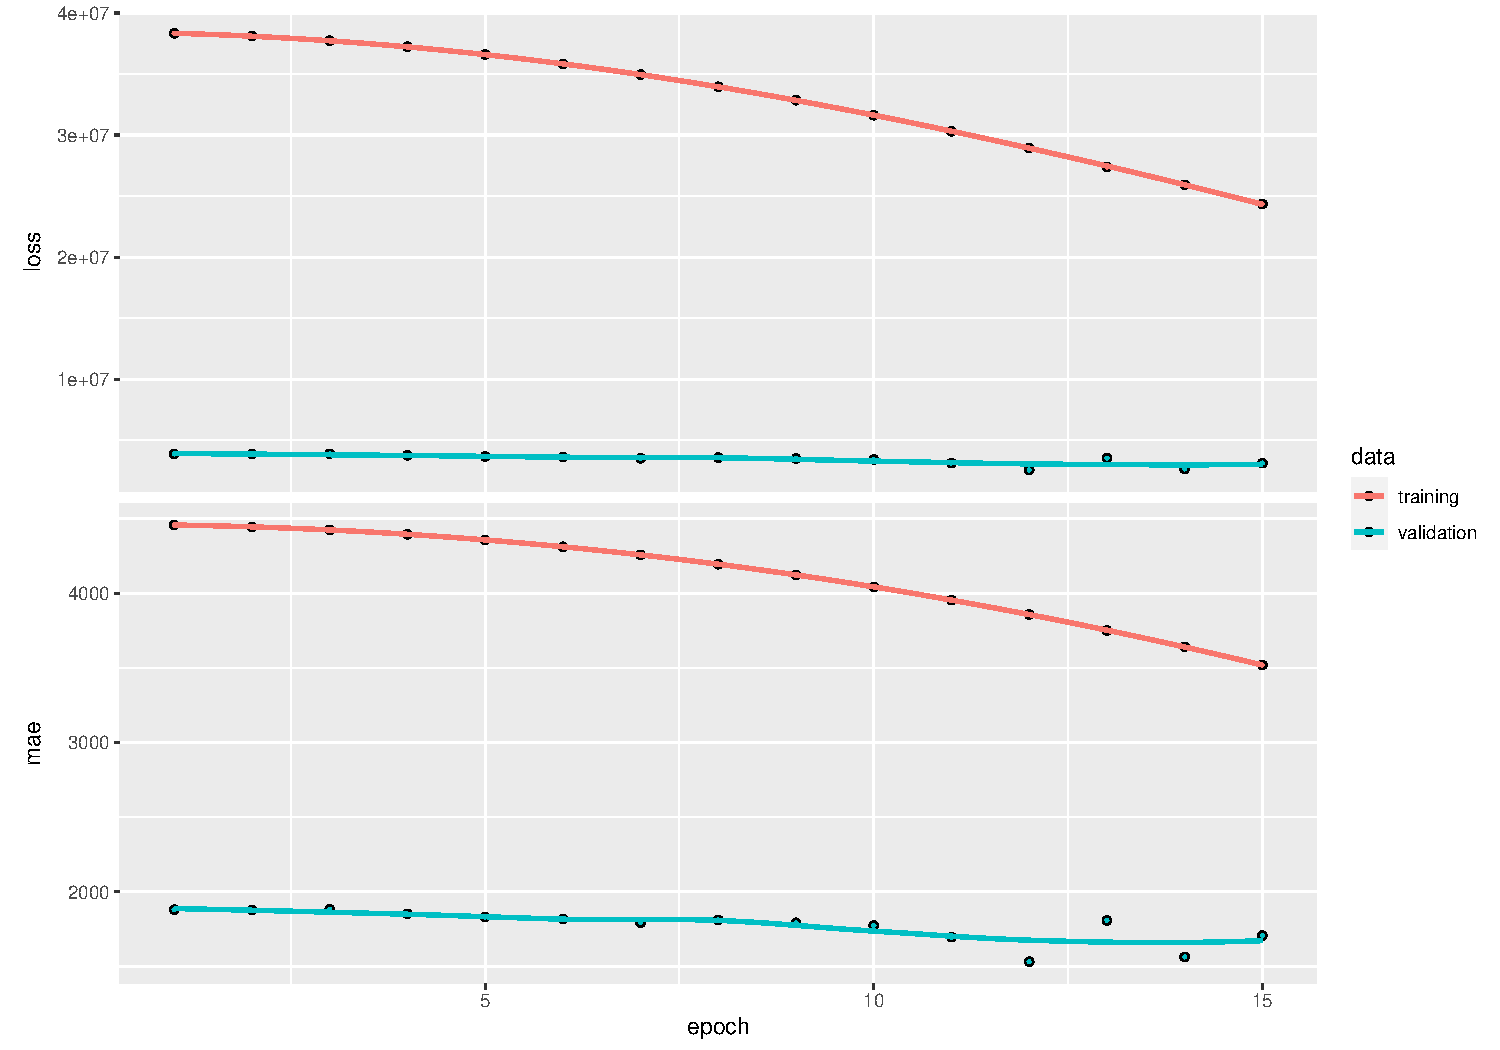
\includegraphics[width=0.6\linewidth,height=0.5\textheight]{figs/unnamed-chunk-21} \end{center}

\normalsize

\end{frame}

\begin{frame}[fragile]{Model Results}
\protect\hypertarget{model-results}{}

\tiny

\begin{Shaded}
\begin{Highlighting}[]
\CommentTok{# Defining the real test features and actual test output.}
\NormalTok{test_features <-}\StringTok{ }\NormalTok{test[, features]}
\NormalTok{test_class <-}\StringTok{ }\NormalTok{test}\OperatorTok{$}\NormalTok{price}

\CommentTok{# Generating predictions for the first 5 records in the test set.}
\NormalTok{model_predictions <-}\StringTok{ }\NormalTok{MLP_model }\OperatorTok\StringTok{ }\KeywordTok{predict}\NormalTok{(}\KeywordTok{as.matrix}\NormalTok{(test_features[}\DecValTok{1}\OperatorTok{:}\DecValTok{5}\NormalTok{,]))}
\NormalTok{model_predictions[model_predictions }\OperatorTok{<}\StringTok{ }\DecValTok{0}\NormalTok{] <-}\StringTok{ }\DecValTok{0}

\CommentTok{# Generating error summary statistic.}
\NormalTok{model_results <-}\StringTok{ }\NormalTok{MLP_model }\OperatorTok\StringTok{ }\KeywordTok{evaluate}\NormalTok{(}\KeywordTok{as.matrix}\NormalTok{(test_features), }\KeywordTok{as.matrix}\NormalTok{(test_class))}
\end{Highlighting}
\end{Shaded}

\normalsize

\end{frame}

\begin{frame}{Hyper-parameter optimization}
\protect\hypertarget{hyper-parameter-optimization}{}

\begin{itemize}
\tightlist
\item
  Determining the optimal hyper-parameters for a machine learning
  algorithm. \vspace{2mm}
\item
  Important for models with large number of hyper-parameters (neural
  networks)

  \begin{itemize}
      \item Random search
      \item Grid search
      \item Bayesian optimization: \texttt{\{rBayesianOptimization,mlrMBO\}}
      \item Genetic algorithm: \texttt{\{GA\}}
    \end{itemize}
   \vspace{2mm}
\item
  An intelligent hyper-parameter search ?
\end{itemize}

\end{frame}

\begin{frame}[fragile]{Bayesian optimization using
\texttt{\{rBayesianOptimization\}}}
\protect\hypertarget{bayesian-optimization-using}{}

\tiny

\begin{Shaded}
\begin{Highlighting}[]
\KeywordTok{library}\NormalTok{(caret)}
\KeywordTok{library}\NormalTok{(rBayesianOptimization)}
\KeywordTok{set.seed}\NormalTok{(}\DecValTok{1234}\NormalTok{)}

\NormalTok{df_households <-}\StringTok{ }\KeywordTok{read.csv}\NormalTok{(}\StringTok{"data/realestate.csv"}\NormalTok{)}
\NormalTok{df_households_filtered <-}\StringTok{ }\NormalTok{df_households[, }\KeywordTok{c}\NormalTok{(}\OperatorTok{-}\DecValTok{1}\NormalTok{,}\OperatorTok{-}\DecValTok{2}\NormalTok{)]}
\KeywordTok{colnames}\NormalTok{(df_households_filtered)[}\DecValTok{6}\NormalTok{] <-}\StringTok{ "price"}
\CommentTok{# Data splitting.}
\NormalTok{data_split <-}\StringTok{ }\KeywordTok{initial_split}\NormalTok{(df_households_filtered, }\DataTypeTok{prop =} \FloatTok{.7}\NormalTok{)}
\NormalTok{train <-}\StringTok{ }\KeywordTok{training}\NormalTok{(data_split)}
\NormalTok{test  <-}\StringTok{ }\KeywordTok{testing}\NormalTok{(data_split)}
\CommentTok{# Define a 10-fold cross validation procedure.}
\NormalTok{train_control <-}\StringTok{ }\KeywordTok{trainControl}\NormalTok{(}\DataTypeTok{method =} \StringTok{"cv"}\NormalTok{, }\DataTypeTok{number =} \DecValTok{5}\NormalTok{)}
\CommentTok{# Defining the fit of the SVM model}
\NormalTok{svm_model_fit <-}\StringTok{ }\ControlFlowTok{function}\NormalTok{(logC, logSigma) \{}
\NormalTok{  model <-}\StringTok{ }\KeywordTok{train}\NormalTok{(price }\OperatorTok{~}\StringTok{ }\NormalTok{., }\DataTypeTok{data =}\NormalTok{ train, }\DataTypeTok{method =} \StringTok{"svmRadial"}\NormalTok{, }\DataTypeTok{metric =} \StringTok{"RMSE"}\NormalTok{,}
                  \DataTypeTok{trControl =}\NormalTok{ train_control,}\DataTypeTok{tuneGrid =} \KeywordTok{data.frame}\NormalTok{(}\DataTypeTok{C =} \KeywordTok{exp}\NormalTok{(logC), }\DataTypeTok{sigma =} \KeywordTok{exp}\NormalTok{(logSigma)))}
  \KeywordTok{list}\NormalTok{(}\DataTypeTok{Score =} \OperatorTok{-}\KeywordTok{getTrainPerf}\NormalTok{(mod)[, }\StringTok{"TrainRMSE"}\NormalTok{], }\DataTypeTok{Pred =} \DecValTok{0}\NormalTok{)}
\NormalTok{\}}
\CommentTok{## Define the bounds and search for hyper-parameters.}
\NormalTok{lower_bounds <-}\StringTok{ }\KeywordTok{c}\NormalTok{(}\DataTypeTok{logC =} \DecValTok{-8}\NormalTok{, }\DataTypeTok{logSigma =} \DecValTok{-10}\NormalTok{)}
\NormalTok{upper_bounds <-}\StringTok{ }\KeywordTok{c}\NormalTok{(}\DataTypeTok{logC =} \DecValTok{15}\NormalTok{, }\DataTypeTok{logSigma =} \FloatTok{-0.65}\NormalTok{)}
\NormalTok{svm_bounds <-}\StringTok{ }\KeywordTok{list}\NormalTok{(}\DataTypeTok{logC =} \KeywordTok{c}\NormalTok{(lower_bounds[}\DecValTok{1}\NormalTok{], upper_bounds[}\DecValTok{1}\NormalTok{]), }\DataTypeTok{logSigma =} \KeywordTok{c}\NormalTok{(lower_bounds[}\DecValTok{2}\NormalTok{], upper_bounds[}\DecValTok{2}\NormalTok{]))}
\CommentTok{# svm_ba_search <- BayesianOptimization(svm_model_fit,}
\CommentTok{#    bounds = svm_bounds,init_grid_dt = NULL, init_points = 0,n_iter = 4, verbose = TRUE)}
\end{Highlighting}
\end{Shaded}

\normalsize

\end{frame}

\begin{frame}{Light Gradient Boosting Machine (LightGBM)}
\protect\hypertarget{light-gradient-boosting-machine-lightgbm}{}

\begin{itemize}
\tightlist
\item
  Gradient boosting framework that uses tree based learning algorithms.
  \vspace{2mm}
\item
  Used for both classification and regression tasks. \vspace{2mm}
\item
  Leading algorithm in many machine learning competitions (Kaggle).
  \vspace{2mm}

  \begin{itemize}
      \item Faster training speed and higher efficiency
      \item Lower memory usage
      \item Highly scalable
      \item Highly parallelizable
      \item Better accuracy than any other boosting algorithms
  \end{itemize}
\end{itemize}

\end{frame}

\begin{frame}[fragile]{LightGBM using \texttt{\{lightgbm\}}}
\protect\hypertarget{lightgbm-using}{}

\tiny

\begin{Shaded}
\begin{Highlighting}[]
\KeywordTok{library}\NormalTok{(lightgbm)}
\KeywordTok{set.seed}\NormalTok{(}\DecValTok{1234}\NormalTok{)}

\KeywordTok{data}\NormalTok{(}\StringTok{"iris"}\NormalTok{)}
\NormalTok{df <-}\StringTok{ }\NormalTok{iris}

\CommentTok{# Data preparation.}
\NormalTok{df}\OperatorTok{$}\NormalTok{Species <-}\StringTok{ }\KeywordTok{as.numeric}\NormalTok{(}\KeywordTok{as.factor}\NormalTok{(df}\OperatorTok{$}\NormalTok{Species)) }\OperatorTok{-}\StringTok{ }\DecValTok{1}
\CommentTok{# Data splitting.}
\NormalTok{data_split <-}\StringTok{ }\KeywordTok{initial_split}\NormalTok{(df, }\DataTypeTok{prop =} \FloatTok{.7}\NormalTok{)}
\NormalTok{train <-}\StringTok{ }\KeywordTok{training}\NormalTok{(data_split)}
\NormalTok{test  <-}\StringTok{ }\KeywordTok{testing}\NormalTok{(data_split)}

\CommentTok{# Transforming to lightgbm data input format.}
\NormalTok{dtrain <-}\StringTok{ }\KeywordTok{lgb.Dataset}\NormalTok{(}\DataTypeTok{data =} \KeywordTok{as.matrix}\NormalTok{(train[}\DecValTok{1}\OperatorTok{:}\DecValTok{4}\NormalTok{]), }\DataTypeTok{label =} \KeywordTok{as.matrix}\NormalTok{(train[,}\DecValTok{5}\NormalTok{]))}
\NormalTok{dtest <-}\StringTok{ }\KeywordTok{lgb.Dataset.create.valid}\NormalTok{(dtrain, }\DataTypeTok{data =} \KeywordTok{as.matrix}\NormalTok{(test[, }\DecValTok{1}\OperatorTok{:}\DecValTok{4}\NormalTok{]), }\DataTypeTok{label =} \KeywordTok{as.matrix}\NormalTok{(test[, }\DecValTok{5}\NormalTok{]))}
\NormalTok{valids <-}\StringTok{ }\KeywordTok{list}\NormalTok{(}\DataTypeTok{test =}\NormalTok{ dtest)}
\CommentTok{# Defining the objective function for a multi-class problem.}
\NormalTok{params <-}\StringTok{ }\KeywordTok{list}\NormalTok{(}\DataTypeTok{objective =} \StringTok{"multiclass"}\NormalTok{, }\DataTypeTok{metric =} \StringTok{"multi_error"}\NormalTok{, }\DataTypeTok{num_class =} \DecValTok{3}\NormalTok{)}

\CommentTok{# Training lightgbm model.}
\NormalTok{lightgbm_model <-}\StringTok{ }\KeywordTok{lgb.train}\NormalTok{(params, dtrain,}\DecValTok{100}\NormalTok{, valids, }\DataTypeTok{min_data =} \DecValTok{1}\NormalTok{,}\DataTypeTok{learning_rate =} \FloatTok{1.0}
\NormalTok{    ,}\DataTypeTok{early_stopping_rounds =} \DecValTok{10}\NormalTok{)}

\CommentTok{# Lightgbm predicts all probabilities for the 3 classes; use argmax() to get the classified class.}
\NormalTok{lightgbm_predictions <-}\StringTok{ }\KeywordTok{predict}\NormalTok{(lightgbm_model, }\KeywordTok{as.matrix}\NormalTok{(test[, }\DecValTok{1}\OperatorTok{:}\DecValTok{4}\NormalTok{]), }\DataTypeTok{reshape =} \OtherTok{TRUE}\NormalTok{)}
\end{Highlighting}
\end{Shaded}

\normalsize

\end{frame}

\begin{frame}{Model Explainability}
\protect\hypertarget{model-explainability}{}

\begin{itemize}
\tightlist
\item
  Majority of the machine learning models are black-box. \vspace{2mm}
\item
  Interpreting and explaining model predictions. \vspace{2mm}
\item
  Explainable machine learning (GDPR law: Right explanation)
  \vspace{2mm}

  \begin{itemize}
      \item Global and Local Interpretable models
      \item \textbf{LIME} (Local Interpretable Model-Agnostic Explanations): \texttt{\{limer\}}
      \item \textbf{SHAP} (SHapley Additive exPlanations): \texttt{\{shapr\}}
      \item \textbf{LORE} (Rule-based Explanations)
      \item \textbf{Anchor}
  \end{itemize}
\end{itemize}

\end{frame}

\begin{frame}[fragile]{Model Explainability using \texttt{\{shapr\}}}
\protect\hypertarget{model-explainability-using}{}

\tiny

\begin{Shaded}
\begin{Highlighting}[]
\KeywordTok{library}\NormalTok{(xgboost)}
\KeywordTok{library}\NormalTok{(shapr)}
\KeywordTok{set.seed}\NormalTok{(}\DecValTok{1234}\NormalTok{)}

\CommentTok{# We are explaining the prediction of household prices.}
\NormalTok{df_households <-}\StringTok{ }\KeywordTok{read.csv}\NormalTok{(}\StringTok{"data/realestate.csv"}\NormalTok{)}
\NormalTok{df_households_filtered <-}\StringTok{ }\NormalTok{df_households[, }\KeywordTok{c}\NormalTok{(}\OperatorTok{-}\DecValTok{1}\NormalTok{,}\OperatorTok{-}\DecValTok{2}\NormalTok{)]}
\KeywordTok{colnames}\NormalTok{(df_households_filtered)[}\DecValTok{6}\NormalTok{] <-}\StringTok{ "price"}

\NormalTok{data_split <-}\StringTok{ }\KeywordTok{initial_split}\NormalTok{(df_households_filtered, }\DataTypeTok{prop =} \FloatTok{.7}\NormalTok{)}
\NormalTok{train <-}\StringTok{ }\KeywordTok{training}\NormalTok{(data_split)}
\NormalTok{test  <-}\StringTok{ }\KeywordTok{testing}\NormalTok{(data_split)}

\NormalTok{features <-}\StringTok{ }\KeywordTok{setdiff}\NormalTok{(}\KeywordTok{names}\NormalTok{(train), }\StringTok{"price"}\NormalTok{)}
\NormalTok{train_features <-}\StringTok{ }\KeywordTok{as.matrix}\NormalTok{(train[, features])}
\NormalTok{train_class <-}\StringTok{ }\KeywordTok{as.matrix}\NormalTok{(train}\OperatorTok{$}\NormalTok{price)}
\NormalTok{test_features <-}\StringTok{ }\KeywordTok{as.matrix}\NormalTok{(test[, features])}

\CommentTok{# Fitting a basic xgboost model to the training data}
\NormalTok{xgboost_model <-}\StringTok{ }\KeywordTok{xgboost}\NormalTok{(}\DataTypeTok{data=}\NormalTok{train_features, }\DataTypeTok{label=}\NormalTok{train_class, }\DataTypeTok{nround=}\DecValTok{10}\NormalTok{, }\DataTypeTok{verbose =} \OtherTok{FALSE}\NormalTok{)}

\CommentTok{# Prepare the data for explanation}
\NormalTok{model_explainer <-}\StringTok{ }\KeywordTok{shapr}\NormalTok{(train_features, xgboost_model)}
\CommentTok{# Expected value without the prediction.}
\NormalTok{expected_price <-}\StringTok{ }\KeywordTok{mean}\NormalTok{(train_class)}
\end{Highlighting}
\end{Shaded}

\normalsize

\end{frame}

\begin{frame}[fragile]{Model Explainability (2)}
\protect\hypertarget{model-explainability-2}{}

\tiny

\begin{Shaded}
\begin{Highlighting}[]
\NormalTok{explanation <-}\StringTok{ }\KeywordTok{explain}\NormalTok{(test_features, }\DataTypeTok{approach =} \StringTok{"empirical"}\NormalTok{, }
                       \DataTypeTok{explainer =}\NormalTok{ model_explainer, }\DataTypeTok{prediction_zero =}\NormalTok{ expected_price)}

\CommentTok{# Plot the resulting explanations for observations 1 and 6}
\KeywordTok{plot}\NormalTok{(explanation, }\DataTypeTok{plot_phi0 =} \OtherTok{FALSE}\NormalTok{, }\DataTypeTok{index_x_test =} \KeywordTok{c}\NormalTok{(}\DecValTok{2}\NormalTok{, }\DecValTok{4}\NormalTok{, }\DecValTok{8}\NormalTok{, }\DecValTok{16}\NormalTok{))}
\end{Highlighting}
\end{Shaded}

\begin{center}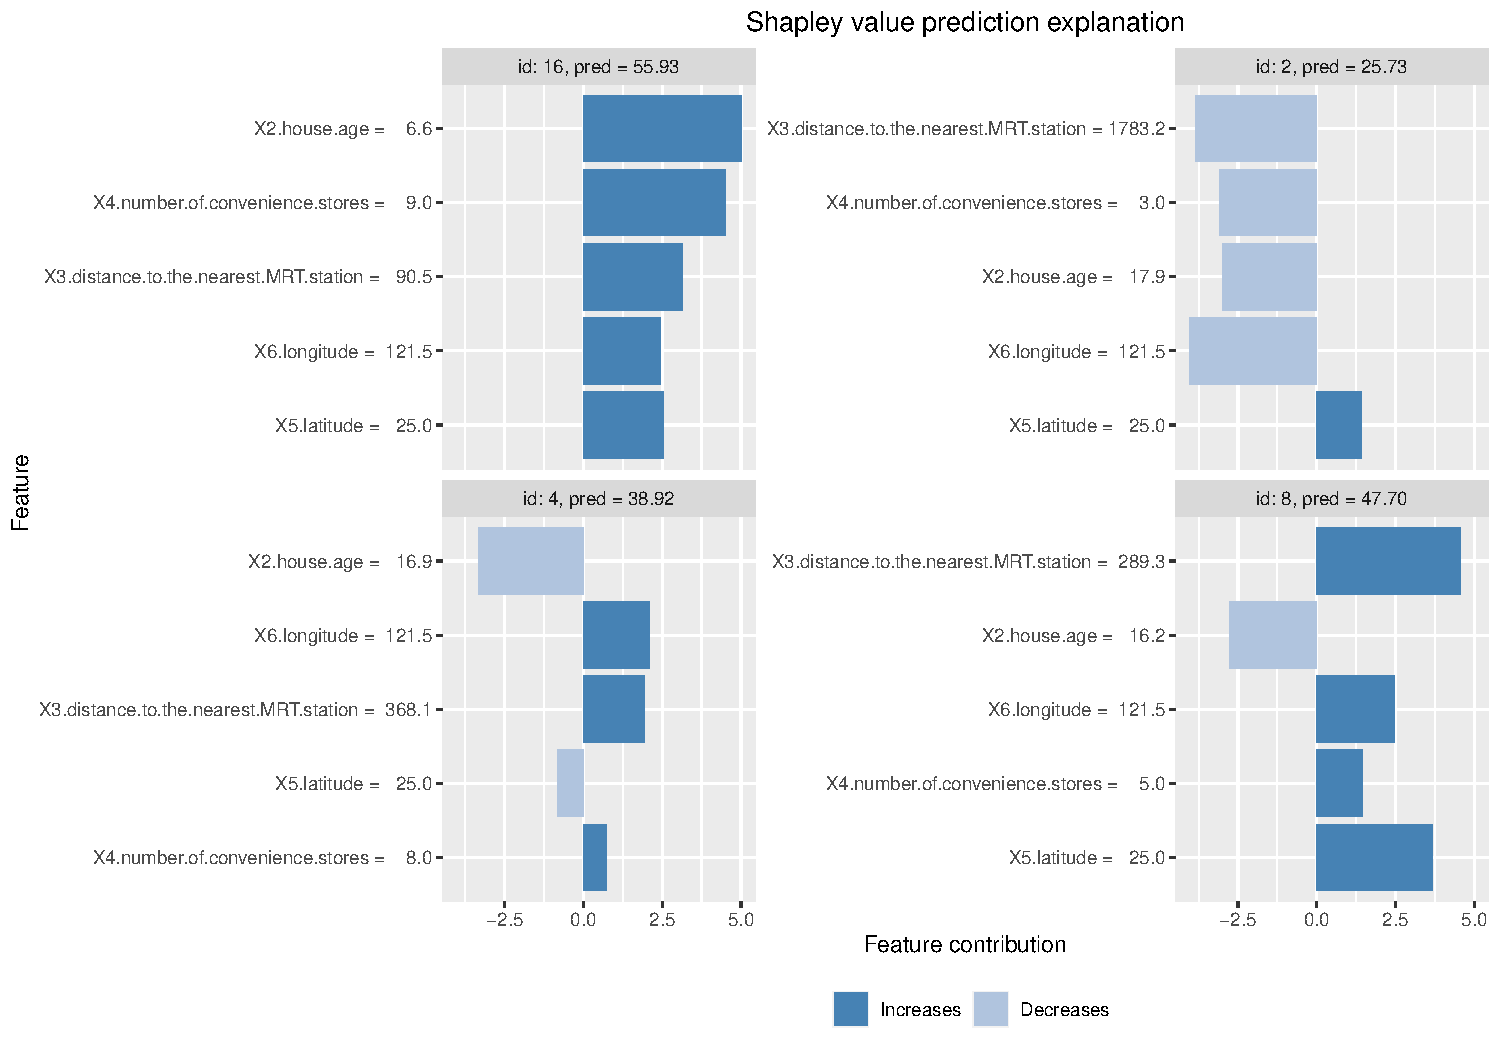
\includegraphics[width=0.8\linewidth,height=0.7\textheight]{figs/unnamed-chunk-26} \end{center}

\normalsize

\end{frame}

\begin{frame}{References}
\protect\hypertarget{references}{}

\tiny

{[}1{]} Hadley Wickham (2021). rvest: Easily Harvest (Scrape) Web Pages.
R package version 1.0.0. \url{https://CRAN.R-project.org/package=rvest}

{[}2{]} Mark van der Loo (2021). simputation: Simple Imputation. R
package version 0.2.6.
\url{https://CRAN.R-project.org/package=simputation}

{[}3{]}
\url{https://cran.r-project.org/web/packages/simputation/vignettes/intro.html}

{[}4{]}
\url{https://www.analyticsvidhya.com/blog/2016/12/introduction-to-feature-selection-methods-with-an-example-or-how-to-select-the-right-variables/}

{[}5{]}
\url{https://www.kaggle.com/zurfer/how-to-use-principle-component-analysis-in-r}

{[}6{]} Miron B. Kursa, Witold R. Rudnicki (2010). Feature Selection
with the Boruta Package. Journal of Statistical Software, 36(11), 1-13.
URL \url{http://www.jstatsoft.org/v36/i11/}

{[}7{]} Max Kuhn (2020). caret: Classification and Regression Training.
R package version 6.0-86. \url{https://CRAN.R-project.org/package=caret}

{[}8{]} Barret Schloerke, Di Cook, Joseph Larmarange, Francois Briatte,
Moritz Marbach, Edwin Thoen, Amos Elberg and Jason Crowley (2021).
GGally: Extension to `ggplot2'. R package version 2.1.1.
\url{https://CRAN.R-project.org/package=GGally}

{[}9{]} Mitchell O'Hara-Wild, Rob Hyndman and Earo Wang (2021). feasts:
Feature Extraction and Statistics for Time Series. R package version
0.1.7. \url{https://CRAN.R-project.org/package=feasts}

{[}10{]} \url{https://rpubs.com/maulikpatel/229337}

\end{frame}

  


\end{document}
